%!TEX program = xelatex

\documentclass[compress]{beamer}
%--------------------------------------------------------------------------
% Common packages
%--------------------------------------------------------------------------

\definecolor{links}{HTML}{663000}
\hypersetup{colorlinks,linkcolor=,urlcolor=links}

\usepackage[english]{babel}
\usepackage{pgfpages} % required for notes on second screen
\usepackage{graphicx}

\usepackage{multicol}

\usepackage{tabularx,ragged2e}
\usepackage{booktabs}

\setlength{\emergencystretch}{3em}  % prevent overfull lines

\usetheme{hri}
\usetikzlibrary{shapes.geometric}
\usetikzlibrary{svg.path}

% Display the navigation bullet even without subsections
\usepackage{remreset}% tiny package containing just the \@removefromreset command
\makeatletter
\@removefromreset{subsection}{section}
\makeatother
\setcounter{subsection}{1}


\newcommand{\source}[2]{{\tiny\it Source: \href{#1}{#2}}}

\usepackage{tikz}
\usetikzlibrary{mindmap,backgrounds,positioning,calc,patterns}

\graphicspath{{figs/}}

\title{Social Signal Processing}
\subtitle{AINT512}
\date{}
\author{Séverin Lemaignan}
\institute{Centre for Neural Systems and Robotics\\{\bf Plymouth University}}

\begin{document}

\licenseframe{github.com/severin-lemaignan/lectures-hri}

\maketitle

\section[Social signals?]{What are Social Signals?}

\videoframe[0.56]{figs/tears-of-steel-extract.mp4}
\imageframe{social-signal}


{
    \paper{Burgoon, Magnenat-Thalmann, Pantic, Vinciarelli, {\bf Social Signal Processing}, 2017}

\begin{frame}{What are social signals?}


    \begin{itemize}
        \item<1-> Social signals are \emph{observable} behaviours that people
            display during social interactions
        \item<2-> Social signals from individual A \emph{produces changes} in others
            (like creating a belief about A, generating an appropriate social
            response, perform an actions)
        \item<3-> the changes are not random, they follow \emph{principles and
            laws} (in particular, \emph{social norms})

    \end{itemize}

\end{frame}
}

\begin{frame}{Why?}
\begin{itemize}

\item The ability to recognize human social signals and social behaviours
  like turn taking, politeness, and disagreement.
\item Essential when building social robots, human-robot interaction,
  interactive systems, \ldots{}
\end{itemize}

    \begin{exampleblock}{3 main problems}

    \begin{itemize}
        \item \emph{Modeling}: identification of the principles and laws
        \item \emph{Analysis}: automatic detection and interpretation
        \item \emph{Synthesis}: automatic generation of artificial social
            signals
    \end{itemize}

    \end{exampleblock}
\end{frame}

\begin{frame}{Is it hard?}

    On the following video, pay particular attention to turn taking
\end{frame}

\videoframe[0.56]{figs/social-signal.mkv}

\begin{frame}{Is it hard?}

As with most human activities that seem easy to us, social signal
processing is tremendously hard.

Often broken down in smaller, sometimes more manageable, tasks:

\begin{itemize}

\item People detection
\item Face detection
\item Face recognition
\item Gesture recognition
\item Gaze detection
\item Facial expression reading (wink, blink, talking, \ldots{})
\item Detection of social signals from verbal communication
\item Emotion recognition (from faces, movement, speech, \ldots{})
\item \ldots{}
\end{itemize}

\end{frame}

\begin{frame}{In this lecture}

\begin{itemize}

\item A historical case study: Kismet.
\item Recognising emotions from speech.
\item Speech recognition in the context of HRI.
\item Classification (k-nearest neighbours and Support Vector Machines)
\item Classification for social signal processing
\end{itemize}

\end{frame}


\begin{frame}{Next 2 weeks}

    More technical:

    \begin{itemize}
        \item How to extract facial features
        \item How to estimate gaze
        \item How to measure attention
        \item How to recognise a face
        \item How to model emotions
    \end{itemize}

\end{frame}

\begin{frame}[plain]
\centering
        \resizebox{!}{0.9\paperheight}{%
            \begin{tikzpicture}[
                    >=latex,
                every edge/.style={<-, draw, very thick}]
        

            \path[small mindmap, 
                level 1 concept/.append style={sibling angle=90}, 
                level 2 concept/.append style={sibling angle=60}, 
            concept color=white,text=hriWarmGreyDark]
            node[concept, visible on=<1-3>] {\bf Social\\Signals...}
            [clockwise from=0]
            child[concept color=hriSec2] { node[concept] (percept){...on the face}
                [clockwise from=30]
                child[concept color=hriSec3Dark,text=white] { node[concept]
                (emotions) {Emotions} }
                child[concept color=hriSec2Dark,text=white] { node[concept] (attention) {Gaze} };
            }
            child[concept color=hriSec2Comp,text=white,visible on=<2->] { node[concept] (knowledge) {...from the body}
                [counterclockwise from=-150]
                child[concept color=hriSec1CompDark,text=white] { node[concept] (soc-rules) {Proxemics} }
                child[concept color=hriSec3Comp,text=black] { node[concept] (soc-ctxt) {Body posture} }
                child[concept color=hriSec2Dark,text=white] { node[concept] (memory) {Gestures} };
            }
            child[concept color=hriSec3Comp,text=black,visible on=<3->] { node[concept] (comm) {...in the voice} 
                [counterclockwise from=90]
                child[concept color=hriSec1CompDark,text=white] { node[concept] (dialog) {Prosody} }
                child[concept color=hriSec3,text=white] { node[concept] (dialog) {Verbal communication} }
                child[concept color=hriSec1Dark,text=white] { node[concept] (non-verbal) {Non-verbal} };
            };


        \end{tikzpicture}
    }
\end{frame}

%%%%%%%%%%%%%%%%%%%%%%%%%%%%%%%%%%%%%%%%%%%%%%%%%%%%%%%%%%%%%%%%%%%%%%%
%%%%%%%%%%%%%%%%%%%%%%%%%%%%%%%%%%%%%%%%%%%%%%%%%%%%%%%%%%%%%%%%%%%%%%%
%%%%%%%%%%%%%%%%%%%%%%%%%%%%%%%%%%%%%%%%%%%%%%%%%%%%%%%%%%%%%%%%%%%%%%%


\section[Kismet]{Case study: Kismet's vision system}


\begin{frame}{Case study: Kismet's vision system}

    \only<1>{
        Remember Kismet?

    \begin{center}
    \video{0.7\paperwidth}{figs/kismet.mp4}
    \end{center}



    Built by Cynthia Breazeal and a team of postgrad students at the
    Massachusetts Institute of Technology (MIT) in 1997.
}
    \only<2>{

        Primary goal: implement an \textbf{attention system}: directing gaze
    towards salient features.

    \begin{itemize}
        \item This should be real-time.
        \item Should resemble the attention system of human infants.
    \end{itemize}

    \begin{columns}
        \begin{column}{0.4\linewidth}
    Attention to several cues:

    \begin{itemize}
        \item Skin tone
        \item Saturated colours
        \item Motion
    \end{itemize}
            
        \end{column}
        \begin{column}{0.6\linewidth}
    \begin{center}
        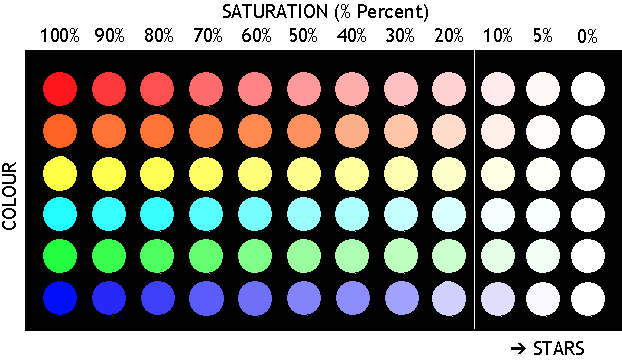
\includegraphics[width=\columnwidth]{colormap}
    \end{center}
        \end{column}
    \end{columns}


    Note that detecting skin tone is easier than detecting faces, and often
    has the same result as face detection
}
\end{frame}

\imageframe{attention}

\begin{frame}{Skin tone feature detector}

    Incoming stream is 8-bit colour images, 128 by 128 pixels\bubblemark{128x128}.


    \bubble<1>[70][0.7][5cm]{128x128}{
  128 x 128 resolution limit caused by hardware throughput and
  computation available at the time, current hardware will be able to
    handle megapixel resolution in real-time.}

    A pixel is \emph{not} skin-toned if:

\begin{itemize}
\item $R < 1.1 G$ and
\item $R < 0.9 B$ and
\item $R > 2.0 \times max(G,B)$ and
\item $R < 20$ and
\item $R > 250$
\end{itemize}

This simple procedure works for most skin colours and under most
lighting conditions.

  It is claimed this even works with non-Caucasian skin, as it picks up
  a colour component in the blood.


\end{frame}

\begin{frame}{Skin tone feature detector}

    \begin{center}
        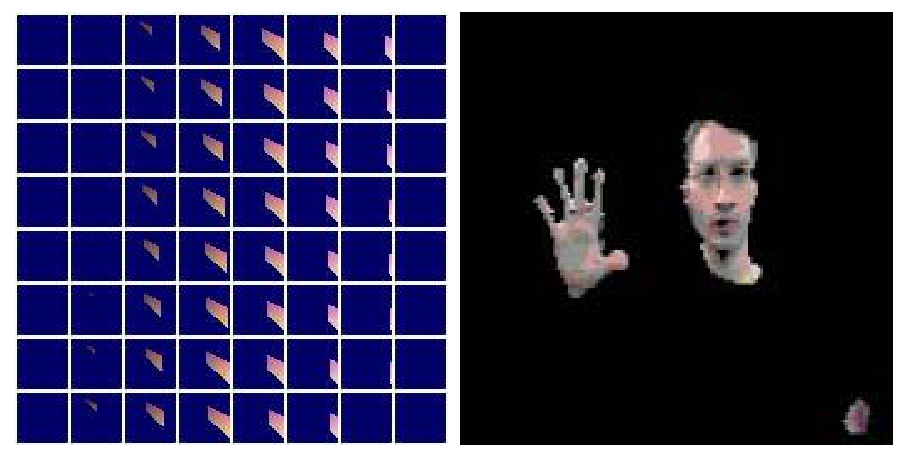
\includegraphics[width=\linewidth]{skin-tone}
    \end{center}

    \begin{columns}
        \begin{column}{0.5\linewidth}
            Cut through RGB 3-dimensional space, picking out only skin tone RGB
            values


        \end{column}
        \begin{column}{0.5\linewidth}
            Result of skin tone detector in action.
        \end{column}
    \end{columns}

\end{frame}

\begin{frame}[fragile]{Saturation detector}

Convert RGB to HSV values

    \begin{columns}
        \begin{column}{0.5\linewidth}
\begin{itemize}

    \item From \texttt{<red, green, blue>} to \texttt{<hue, saturation, value>} representation.
\item \textbf{hue} is the ``colour'', \textbf{saturation} is how deep the
  colour is and \textbf{value} is how bright the pixel is.
\item Usually an excellent first step in computer vision when processing
  colour images, as it removes the effect of uneven lighting.
\end{itemize}
            
        \end{column}
        \begin{column}{0.5\linewidth}

    \begin{center}
        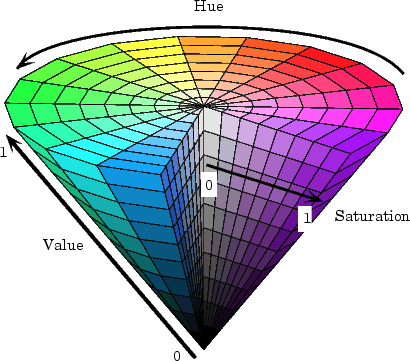
\includegraphics[width=\columnwidth]{hsv}
    \end{center}

        \end{column}
    \end{columns}


\end{frame}

\begin{frame}[fragile]{RGB to HSV in Python}

    \begin{columns}
        \begin{column}{0.5\linewidth}
\begin{pythoncode}
def rgb2hsv(r, g, b):
    r, g, b = r/255.0, g/255.0, b/255.0
    mx = max(r, g, b)
    mn = min(r, g, b)
    df = mx-mn
    if mx == mn:
        h = 0
    elif mx == r:
        h = (60 * ((g-b)/df) + 360) % 360
    elif mx == g:
        h = (60 * ((b-r)/df) + 120) % 360
    elif mx == b:
        h = (60 * ((r-g)/df) + 240) % 360
    if mx == 0:
        s = 0
    else:
        s = df/mx
    v = mx
    return h, s, v
\end{pythoncode}
\source{http://code.activestate.com/recipes/576919-python-rgb-and-hsv-conversion/}{Python recipes}
            
        \end{column}
        \begin{column}{0.5\linewidth}
            \vspace{4cm}

or better:

\begin{pythoncode}
import colorsys
colorsys.rgb_to_hsv(0.2, 0.4, 0.4)
--> (0.5, 0.5, 0.4)
colorsys.hsv_to_rgb(0.5, 0.5, 0.4)
--> (0.2, 0.4, 0.4)
\end{pythoncode}

        \end{column}
    \end{columns}


\end{frame}

\begin{frame}[fragile]{Saturation detector}

\begin{itemize}

\item Convert image from RGB to HSV, and mark pixels (by setting them to
  WHITE) that have a saturation over a certain threshold.
\item Focus on \textbf{Centre of Gravity} of all saturation pixels.
\end{itemize}

\begin{matlabcode}
void centerOfGravity (int[][] image, int imageWidth,
        int imageHeight)
{
    int SumX = 0;
    int SumY = 0;
    int num = 0;
    for (int i=0; i&lt;imageWidth; i++)
    {
        for (int j=0; j&lt;imageHeight; j++)
        {
            if (image[i][j] == WHITE)
            {
                SumX = SumX + i;
                SumY = SumY + j;
                num++;
            }
        }
    }
    SumX = SumX / num;
    SumY = SumY / num;
    // The coordinate (SumX,SumY) is the center of gravity
}
\end{matlabcode}

\end{frame}

\begin{frame}[fragile]{Motion detector}

\begin{itemize}

\item Motion is a strong social signal, essential for survival (both in
  detecting prey and predator). Robots are expected to be sensitive to
  motion as well.
\end{itemize}

\begin{matlabcode}
int[][] motionDetection (int[][] image,
        int[][] imagePrevious, int imageWidth, int
        imageHeight)

{
    int[][] imageMotion;
    int num = 0;
    imageMotion = (int\\)malloc( imageWidth \ imageHeight)

    for (int i=0; i&lt;imageWidth; i++)
    {
        for (int j=0; j&lt;imageHeight; j++)
        {
            imageMotion[i][j] = abs(image[i][j] - imagePrevious[i][j]);
        }
    }
}
\end{matlabcode}

\end{frame}

\begin{frame}{Optical flow}

    Today, motion detection is performed by computing the \emph{optical flow}
    of a video stream.

    \video{0.8\paperwidth}{figs/optical_flow.mp4}

    The colours indicate the direction in which each pixel moves.


\end{frame}


\begin{frame}{Post-attentive processing}

After attention has been fixed, run some additional algorithms

\begin{itemize}

\item Eye detection: using template matching.
\item Proximity estimation: using stereo vision.
\item Loom detection: if the size of the motion blob increases rapidly.
\item Threat detection: rapid motion or fast looming.
\end{itemize}

The results of these visual processes feed into the behaviour manager of
the robot.

\begin{itemize}

\item Robot focuses on visual regions that draw its attention
\end{itemize}

\end{frame}

\begin{frame}{Selection of attention}

Kismet does not attend to all three features for computational
reasons\bubblemark{processingpower}, but selects one according to its
current behaviour.

For example, when the {\tt seek\_people} behaviour is active, it uses skin tone
to direct its attention.

\bubble<1>[110][1.7][5cm]{processingpower}{ This was back in early 2000s.
Current hardware can handle this computational load without problem.
However, it is good practice to not spend processor cycles on signals you
do not require.  }

    \onslide<2>{
Implementation: an \textbf{attention activation map}

\begin{itemize}
    \item A 128 by 128 map of activation for the feature detectors is
    constructed.
    \item A threshold is applied to get rid of noise.
    \item Connected regions are found using the 4-connect algorithm.
    \item Regions of less than 30 pixels are thrown away.
    \item Centroid is computed.
    \item Attention is drawn to largest region.
\end{itemize}

The attention map is independent of the feature (color, motion, \ldots{})
}

\end{frame}

\begin{frame}{The auditory system}

Kismet does not understand human language!

It only pays attention to emotional content of speech. This is done
though monitoring \textbf{prosody}.

Advantages:

\begin{itemize}

\item rather easy and computationally inexpensive
\item the robot is not committed to one single language
\item the robot is speaker independent
\end{itemize}

\end{frame}

\begin{frame}{Emotion from prosody}

„Sie haben es gerade hochgetragen und jetzt gehen sie wieder runter``
(They just carried it upstairs and now they are going down again).

    \begin{center}
    \video[1]{1cm}{figs/prosody/media1.mp4}\hspace{0.3em}
    \video[1]{1cm}{figs/prosody/media2.mp4}\hspace{0.3em}
    \video[1]{1cm}{figs/prosody/media3.mp4}\hspace{0.3em}
    \video[1]{1cm}{figs/prosody/media4.mp4}\hspace{0.3em}
    \video[1]{1cm}{figs/prosody/media5.mp4}
    \end{center}

    \source{http://emodb.bilderbar.info/start.html}{Berlin Database of
  Emotional Speech}


Which emotion do you recognise?


    \textbf{Anger} -- \textbf{Boredom} -- \textbf{Disgust} -- \textbf{Anxiety/Fear} -- \textbf{Happiness} --
    \textbf{Sadness} --  \textbf{Neutral}

Humans recognise emotions from prosody with approx. 80\% accuracy
(\textit{caveat: this is for speech spoken by actors in a recording studio})

\end{frame}

\begin{frame}{Speech processing system}

Compute features from the samples

\begin{itemize}

\item Pitch mean
\item Pitch variance
\item Maximum pitch.
\item Minimum pitch.
\item Pitch range.
\item \ldots{}
\end{itemize}

    \begin{center}
        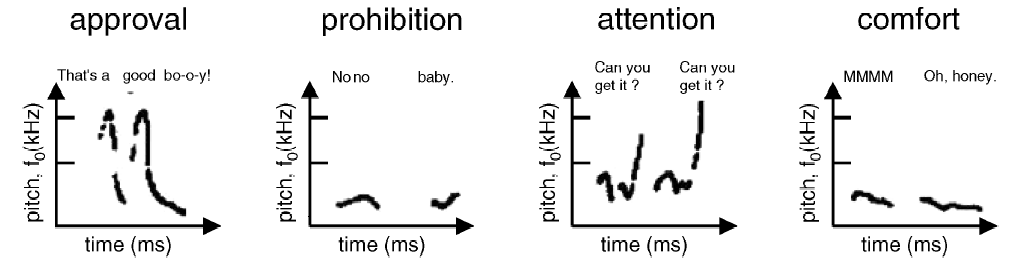
\includegraphics[width=0.8\linewidth]{prosody}
    \end{center}

\end{frame}

\begin{frame}{Audio processing stream in Kismet}

    Many different samples were recorded and classified by a human subject.
    Then an algorithm was trained (Expectation Maximisation) to classify the
    samples into five distinct classes.

    \begin{itemize}
        \item Approvals
        \item Attention drawing
        \item Prohibition
        \item Comforting
        \item Neutral
    \end{itemize}

    \begin{center}
        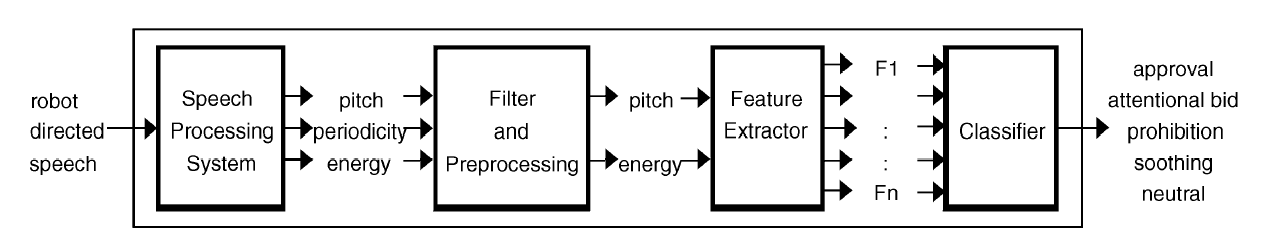
\includegraphics[width=0.8\linewidth]{kismet-audio-processing}
    \end{center}

\end{frame}

%%%%%%%%%%%%%%%%%%%%%%%%%%%%%%%%%%%%%%%%%%%%%%%%%%%%%%%%%%%%%%%%%%%%%%%
%%%%%%%%%%%%%%%%%%%%%%%%%%%%%%%%%%%%%%%%%%%%%%%%%%%%%%%%%%%%%%%%%%%%%%%
%%%%%%%%%%%%%%%%%%%%%%%%%%%%%%%%%%%%%%%%%%%%%%%%%%%%%%%%%%%%%%%%%%%%%%%


\section{Speech recognition}

\begin{frame}{Speech recognition}

    See Guido's lectures, but here's a small heads up.

    Automated Speech Recognition has improved tremendously over the past few
    years.

    \begin{itemize}
        \item Improved recognition performance
        \item Speaker independence
        \item Can deal with a larger amount of background noise
    \end{itemize}

    Plenty of reports on increased performance

\begin{itemize}

\item ``\href{https://blogs.microsoft.com/next/2016/10/18/historic-achievement-microsoft-researchers-reach-human-parity-conversational-speech-recognition/\#g5qKXHrZZ2pbxuPH.99}{Historic
  Achievement: Microsoft researchers reach human parity in
  conversational speech recognition}'' (Oct 2016)
\item Error rate (\% of misunderstood words) on
  \href{https://catalog.ldc.upenn.edu/LDC2004S13}{Switchboard} (SWB) and
  CallHome (CH) corpus.
\end{itemize}

    \begin{center}
        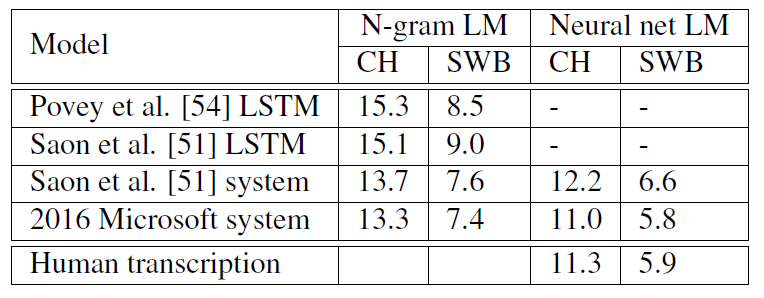
\includegraphics[width=0.8\linewidth]{asr-error-rates}
    \end{center}

\end{frame}

\begin{frame}{Speech recognition}

So what has changed?

\begin{itemize}

\item Introduction of new models for speech recognition based on Deep Neural
  Networks (DNN) or Convolutional Neural Networks (CNN), replacing
  models based on n-grams or Hidden Markov Models (HMM).

        \begin{center}
            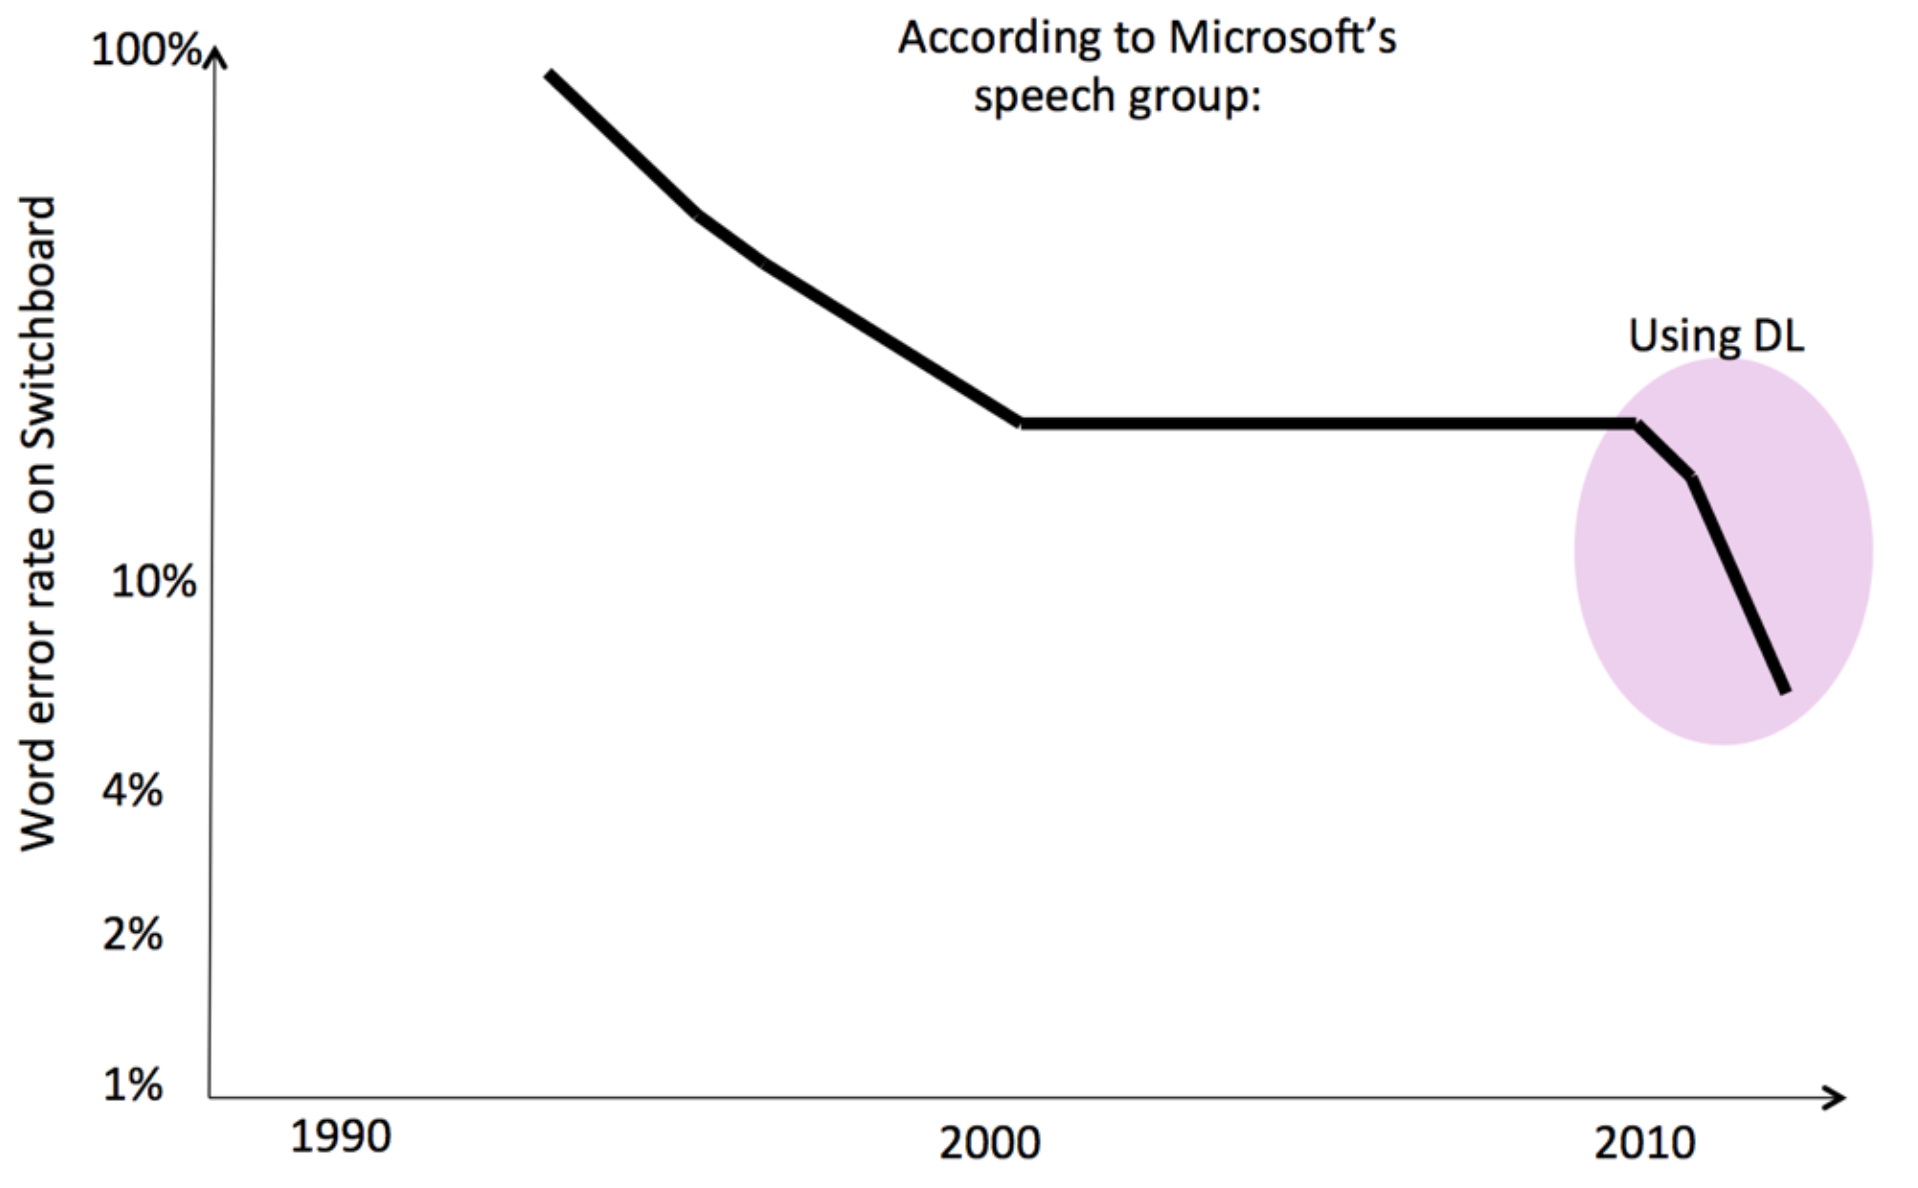
\includegraphics[width=0.8\linewidth]{asr-evolution}
        \end{center}
\item More availability of training data, often collected through speech
  command interfaces (such as Google Now, Microsoft's Xbox chat
  function).
\item Computational power to train DNN has increased: High Performance
  Computing clusters and Graphical Processing Units (GPUs).
\item Recognition happens in the cloud, rather than on-board a device. This
  offers more computational power and access to large networks.
\end{itemize}

\end{frame}

\imageframe[caption=Open-source efforts by Mozilla]{common-voice-project}

\begin{frame}{Speech recognition}

Question

\begin{itemize}

\item So, given that ASR performance seems high, how good is it really for
  Human-Robot Interaction?
\end{itemize}

Human-Robot Interaction is unique

\begin{itemize}

\item There is often a noise environment.
\item Users are at a distance from the robot (and any speakers carried on
  the robot). Almost all ASR engines have been trained on speech
  recorded close to the microphone (\textless{} 10cm).
\item There might be a multi-party conversation (i.e.~multiple speakers).
\end{itemize}

\end{frame}

\begin{frame}{Speech recognition for children}

How well does speech recognition perform for child speech?

\begin{itemize}

\item For counting (1,2,3, \ldots{}) and short sentences \textbf{spoken by
  adults}, recognition rate is \textbf{90\% using Nao microphone and
  on-board ASR} (Nuance VoCon 4.7). And up to 99\% recognition with a
  high-quality microphone and Google ASR.
\item Can we assume that ASR on children's speech will have the same
  performance?
\end{itemize}

Child speech is very different from adult speech.

\begin{itemize}

\item Higher pitch (due to small vocal tracts).
\item higher number of disfluencies and, especially in younger children,
  language utterances are often ungrammatical (e.g. ``The boy
  \emph{putted} the frog in the box'').
\end{itemize}

\end{frame}

\imageframe{child-speech}

\begin{frame}{Examples of recordings (cleaned-up, normalised)}

\begin{itemize}

\item Numbers (0 to 10)
\item Sentences
\item Spontaneous speech
\end{itemize}

Jacob, native English speaker

Julia, native English speaker

Clean

Noisy

(Recorded with studio microphone)

\end{frame}

\begin{frame}{Impact of microphone type}

    \begin{center}
        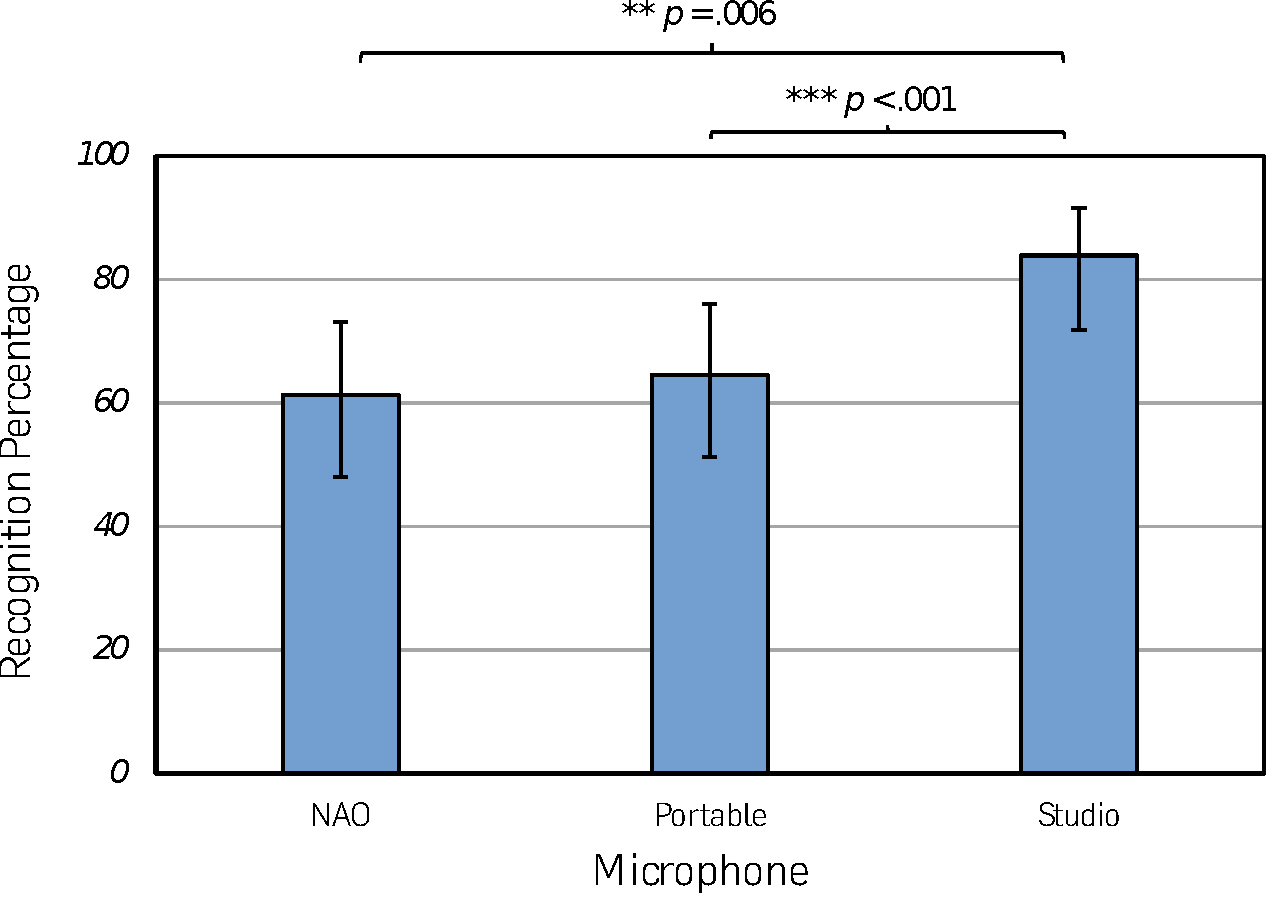
\includegraphics[width=0.8\linewidth]{mic_graph}
    \end{center}

Recognition rate of numbers spoken by children, split by microphone type
(62 utterances) using Nao's ASR engine (Nuance Vocon 4.7) constrained by
a grammar containing only number words.

\end{frame}

\begin{frame}{Impact of background noise}

\begin{center}
    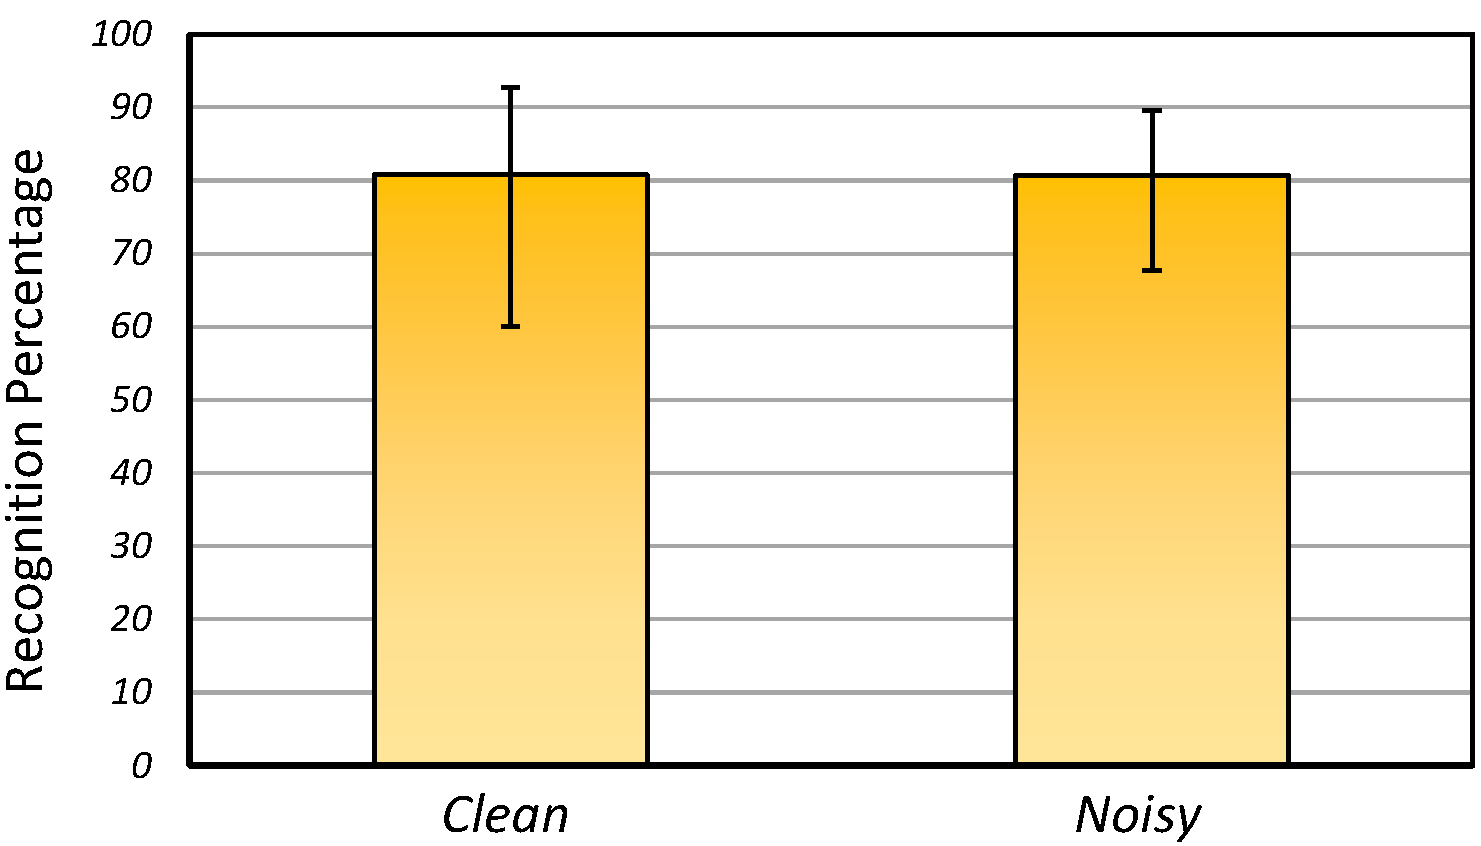
\includegraphics[width=0.8\linewidth]{noise_graph}
\end{center}

Recognition rate of number utterances spoken by children, split by
background noise level (83 total utterances) using Nao's ASR engine
(Nuance Vocon 4.7) constrained by a grammar containing only number
words.

Clean

Background noise

\end{frame}

\begin{frame}{Location of speaker wrt. Nao}

\only<1>{
    \begin{columns}
        \begin{column}{0.5\linewidth}
            \begin{center}
                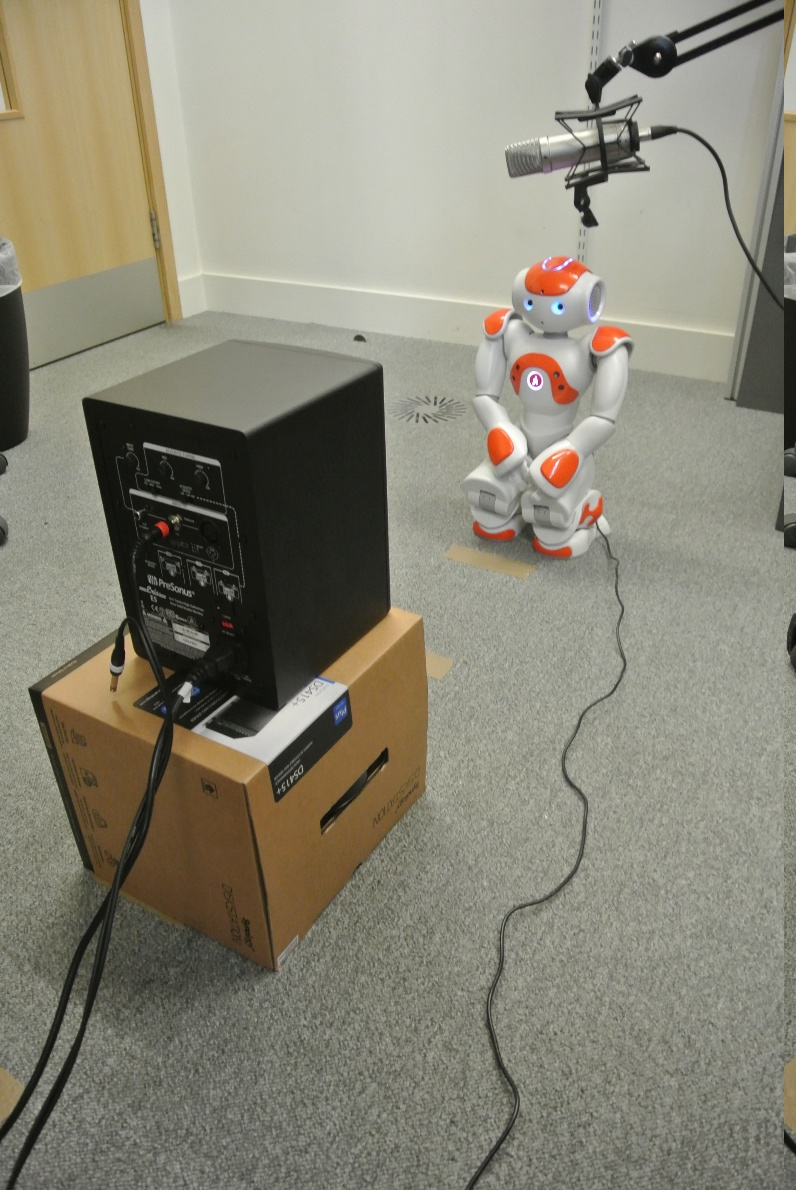
\includegraphics[width=0.8\linewidth]{recording-audio-nao}
            \end{center}
        \end{column}
        \begin{column}{0.5\linewidth}
    \begin{center}
        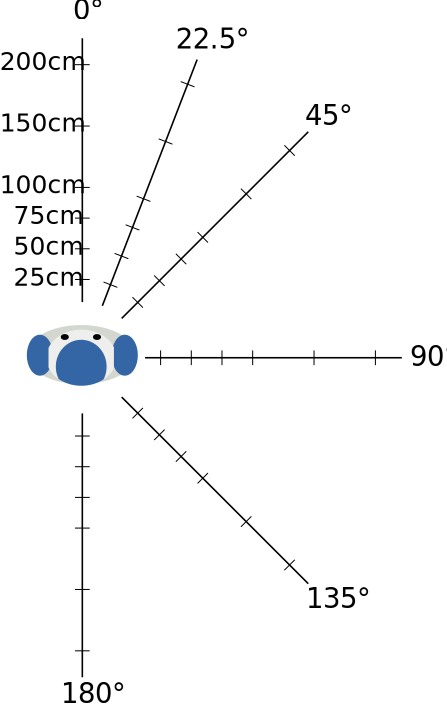
\includegraphics[width=0.8\linewidth]{directional_recordings}
    \end{center}
        \end{column}
    \end{columns}

}

    \only<2>{
        \begin{center}
            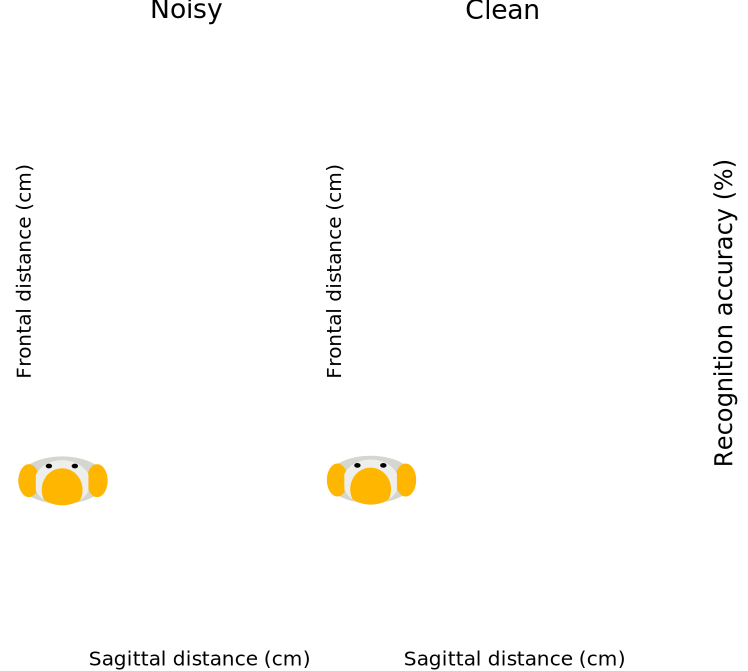
\includegraphics[width=0.8\linewidth]{heatmaps}
        \end{center}
    }


\end{frame}

%%%%%%%%%%%%%%%%%%%%%%%%%%%%%%%%%%%%%%%%%%%%%%%%%%%%%%%%%%%%%%%%%%%%%%%
%%%%%%%%%%%%%%%%%%%%%%%%%%%%%%%%%%%%%%%%%%%%%%%%%%%%%%%%%%%%%%%%%%%%%%%
%%%%%%%%%%%%%%%%%%%%%%%%%%%%%%%%%%%%%%%%%%%%%%%%%%%%%%%%%%%%%%%%%%%%%%%


\section{Classification}

\begin{frame}{Classification}

Social signal processing often relies on \textbf{classification.}

\begin{itemize}
    \item \href{https://en.wikipedia.org/wiki/Statistical_classification}{\textbf{Classification}}
        is deciding on which \textbf{category} a new observation belongs to
        based on training data.

    \item The training data contains data and known categories.
    \item Classification is a \textbf{supervised} learning algorithm.
\end{itemize}

\pause

Examples:

\begin{itemize}

\item An incoming tweet needs to classified as being positive or negative.
\item An radar ping of a flying objects needs to be classified as belonging
  to one of \emph{n} possible planes.
\item The prosody of speech needs to be classified as belonging to one of
  six basic categories of emotion (happy, sad, angry, bored, surprised,
  neutral).
\item A gesture filmed through a camera needs to be classified as meaning
  stop, go, left or right.
\end{itemize}

\end{frame}

\begin{frame}{Classification: example}

\begin{itemize}
\item Two dimensional problem
\item Two categories, with training data for both categories
\item To which category does a new observation belong?
\end{itemize}

    \begin{center}
        \resizebox{0.5\linewidth}{!}{
            \begin{tikzpicture}[>=latex,
                starmarker/.style={star, fill=hriSec2Comp,opacity=0.5,inner sep=0,minimum size=4pt}]

                %\draw[help lines] (0,0) grid (5,4);
                \draw[thick, ->] (0,0) -> (5.2,0);
                \draw[thick, ->] (0,0) -> (0,4.2);

                \fill [hriSec2, opacity=0.5] (2.2,1.3) circle (2pt);
                \fill [hriSec2, opacity=0.5] (3.2,2.3) circle (2pt);
                \fill [hriSec2, opacity=0.5] (2.5,0.4) circle (2pt);
                \fill [hriSec2, opacity=0.5] (0.6,0.3) circle (2pt);
                \fill [hriSec2, opacity=0.5] (2.8,0.7) circle (2pt);
                \fill [hriSec2, opacity=0.5] (3.8,1.7) circle (2pt);
                \fill [hriSec2, opacity=0.5] (4.5,1.0) circle (2pt);

                \only<1-2,4->{
                    \fill [hriSec2, opacity=0.5] (4.1,2.4) circle (2pt);
                    \fill [hriSec2, opacity=0.5] (4.5,3.5) circle (2pt);
                }

                \fill [hriSec3Comp, opacity=0.5] (2.3,3.2) rectangle +(3.5pt,3.5pt);
                \fill [hriSec3Comp, opacity=0.5] (0.3,0.6) rectangle +(3.5pt,3.5pt);
                \fill [hriSec3Comp, opacity=0.5] (1.5,1.4) rectangle +(3.5pt,3.5pt);
                \fill [hriSec3Comp, opacity=0.5] (2.4,2.2) rectangle +(3.5pt,3.5pt);
                \fill [hriSec3Comp, opacity=0.5] (0.7,2.8) rectangle +(3.5pt,3.5pt);
                \fill [hriSec3Comp, opacity=0.5] (1.7,3.8) rectangle +(3.5pt,3.5pt);
                \fill [hriSec3Comp, opacity=0.5] (1.0,2.5) rectangle +(3.5pt,3.5pt);

                \only<1-3>{
                    \fill [hriSec3Comp, opacity=0.5] (2.2,2.5) rectangle +(3.5pt,3.5pt);
                    \fill [hriSec3Comp, opacity=0.5] (1.3,2.2) rectangle +(3.5pt,3.5pt);
                }
                \only<4->{
                    \fill [hriSec2, opacity=0.5] (2.2,2.5) circle (2pt);
                    \fill [hriSec2, opacity=0.5] (1.3,2.2) circle (2pt);
                }


                \only<1>{
                    \fill (3.5,3) circle (2pt) node[above] {?};
                }

                \only<2>{
                    \draw[dashed, ultra thick] (0,0.1) -- (4.9,4);
                    \fill[hriSec3Comp] (3.5,3) circle (3pt);
                }

                \only<3->{
                \node[starmarker] at(2.8,3.5) {};
                \node[starmarker] at(3.2,2.6) {};
                \node[starmarker] at(3.7,2.5) {};
                \node[starmarker] at(4.8,2.3) {};
                \node[starmarker] at(4.2,3.5) {};
                \node[starmarker] at(4.7,3.2) {};
                \node[starmarker] at(3.6,3.5) {};
                \node[starmarker] at(3.2,3.0) {};
            }

                \only<3>{
                \coordinate (center) at (3,2.5);
                    \draw[dashed, ultra thick] (0,0.1) -- (center);
                    \draw[dashed, ultra thick] (2.1,4) -- (center);
                    \draw[dashed, ultra thick] (5,2) -- (center);
                }

                \only<4>{
                    \draw[ultra thick, dashed] svg[scale=0.355mm] {M 0,0 C 7.3028978,5.4871928 17.986558,18.924336 25.712718,23.631806 33.180198,27.981126 42.096418,29.772386 48.918988,35.157436 53.234728,39.486306 53.152318,48.037756 47.022748,50.669426 42.040828,52.174296 36.443098,53.302996 33.138128,57.811566 29.262578,61.437306 31.018648,68.735086 36.313848,69.650946 45.513978,70.336506 52.317528,79.815856 61.890318,78.092016 67.994798,76.405086 66.315798,68.913296 65.206548,64.346256 62.816378,59.430726 65.265748,53.196516 71.506418,55.666566 76.735423,57.642746 77.207603,62.923806 82.494663,67.005556 87.781723,71.087306 97.769793,65.300896 103.85227,64.480036 109.93475,63.659176 113.08322,69.782766 115.38846,74.251266 119.51535,82.521786 120.32667,91.925786 123.66302,100.4599 126.136,107.56288 135.65151,102.31662 131.03155,96.353476 128.47853,90.355456 123.56513,84.297766 125.88953,77.387966 127.40319,68.340166 132.79437,57.935476 141.71719,53.730616};
                    \draw[ultra thick, dashed] svg[scale=0.355mm] {M 84.116373,67.870526 C 84.388083,71.283156 84.773743,74.838716 83.492033,78.110256 82.006413,83.150896 79.611653,88.027626 75.899043,91.805036 73.482483,94.619536 71.510448,97.822816 70.142548,101.27341 69.330828,105.09004 70.025558,108.99486 70.135548,112.8405};
                }



            \end{tikzpicture}
        }
    \end{center}


    \only<2> {
        When categories can be linearly separated, we have a very easy
        classification problem.
    }

    \only<3> {
        Three or more can still be linearly separated.
    }


    \only<4-> {
        \textbf{But what if categories are not linearly separable?}
    }

\end{frame}

\begin{frame}{Two classification methods}

Two methods will be explained here:

\begin{itemize}

\item $k$-nearest Neighbours (kNN)
\item Support Vector Machines (SVM)
\end{itemize}

But there are hundreds of classifiers

\begin{itemize}

\item Decision trees
\item Random forest
\item Bayes classifiers
\item Neural Networks
\item \ldots{}
\end{itemize}

\end{frame}

\begin{frame}{$k$-nearest Neighbours}


When an observation comes in, calculate the distance to the $k$ nearest
neighbours. The observation belongs to the class the most frequent amongst neighbours.

    \begin{center}
        \resizebox{0.5\linewidth}{!}{
            \begin{tikzpicture}[>=latex,
                starmarker/.style={star, fill=hriSec2Comp,opacity=0.5,inner sep=0,minimum size=4pt}]

                %\draw[help lines] (0,0) grid (5,4);
                \draw[thick, ->] (0,0) -> (5.2,0);
                \draw[thick, ->] (0,0) -> (0,4.2);

                \fill [hriSec2, opacity=0.5] (2.2,1.3) circle (2pt);
                \fill [hriSec2, opacity=0.5] (3.2,2.3) circle (2pt);
                \fill [hriSec2, opacity=0.5] (2.5,0.4) circle (2pt);
                \fill [hriSec2, opacity=0.5] (0.6,0.3) circle (2pt);
                \fill [hriSec2, opacity=0.5] (2.8,0.7) circle (2pt);
                \fill [hriSec2, opacity=0.5] (3.8,1.7) circle (2pt);
                \fill [hriSec2, opacity=0.5] (4.5,1.0) circle (2pt);

                \fill [hriSec2, opacity=0.5] (1.3,2.2) circle (2pt);
                \fill [hriSec2, opacity=0.5] (4.1,2.4) circle (2pt);
                \fill [hriSec2, opacity=0.5] (4.5,3.5) circle (2pt);
                \fill [hriSec2, opacity=0.5] (2.2,2.5) circle (2pt);

                \fill [hriSec3Comp, opacity=0.5] (2.3,3.2) rectangle +(3.5pt,3.5pt);
                \fill [hriSec3Comp, opacity=0.5] (0.3,0.6) rectangle +(3.5pt,3.5pt);
                \fill [hriSec3Comp, opacity=0.5] (1.5,1.4) rectangle +(3.5pt,3.5pt);
                \fill [hriSec3Comp, opacity=0.5] (2.4,2.2) rectangle +(3.5pt,3.5pt);
                \fill [hriSec3Comp, opacity=0.5] (0.7,2.8) rectangle +(3.5pt,3.5pt);
                \fill [hriSec3Comp, opacity=0.5] (1.7,3.8) rectangle +(3.5pt,3.5pt);
                \fill [hriSec3Comp, opacity=0.5] (1.0,2.5) rectangle +(3.5pt,3.5pt);



                \node[starmarker] at(2.8,3.5) {};
                \node[starmarker] at(3.2,2.6) {};
                \node[starmarker] at(3.7,2.5) {};
                \node[starmarker] at(4.8,2.3) {};
                \node[starmarker] at(4.2,3.5) {};
                \node[starmarker] at(4.7,3.2) {};
                \node[starmarker] at(3.6,3.5) {};
                \node[starmarker] at(3.2,3.0) {};

                \only<1>{
                    \fill (3.5,3) circle (2pt);
                }
                \only<2>{
                    \node[starmarker,opacity=1] at(3.5,3) {};
                    \fill (1.5,3) circle (2pt);
                }
                \only<3>{
                    \node[starmarker,opacity=1] at(3.5,3) {};
                    \fill [hriSec3Comp, opacity=1] (1.5,3) rectangle +(3.5pt,3.5pt);
                    \fill (1.8,1.9) circle (2pt);
                }
                \only<4>{
                    \node[starmarker,opacity=1] at(3.5,3) {};
                    \fill [hriSec3Comp, opacity=1] (1.5,3) rectangle +(3.5pt,3.5pt);
                    \fill (1.8,1.9) circle (2pt) node[above] {?};
                    %\fill [hriSec3Comp, opacity=1] (1.8,1.9) rectangle +(3.5pt,3.5pt);
                }


            \end{tikzpicture}
        }
    \end{center}

\end{frame}
\begin{frame}{Choosing $k$}


\begin{itemize}
    \item too small and it sensitive to classification noise.
    \item too large and classification accuracy decreases.
\end{itemize}

Decision border with $k=1$ and $k=2$:

    \begin{center}
        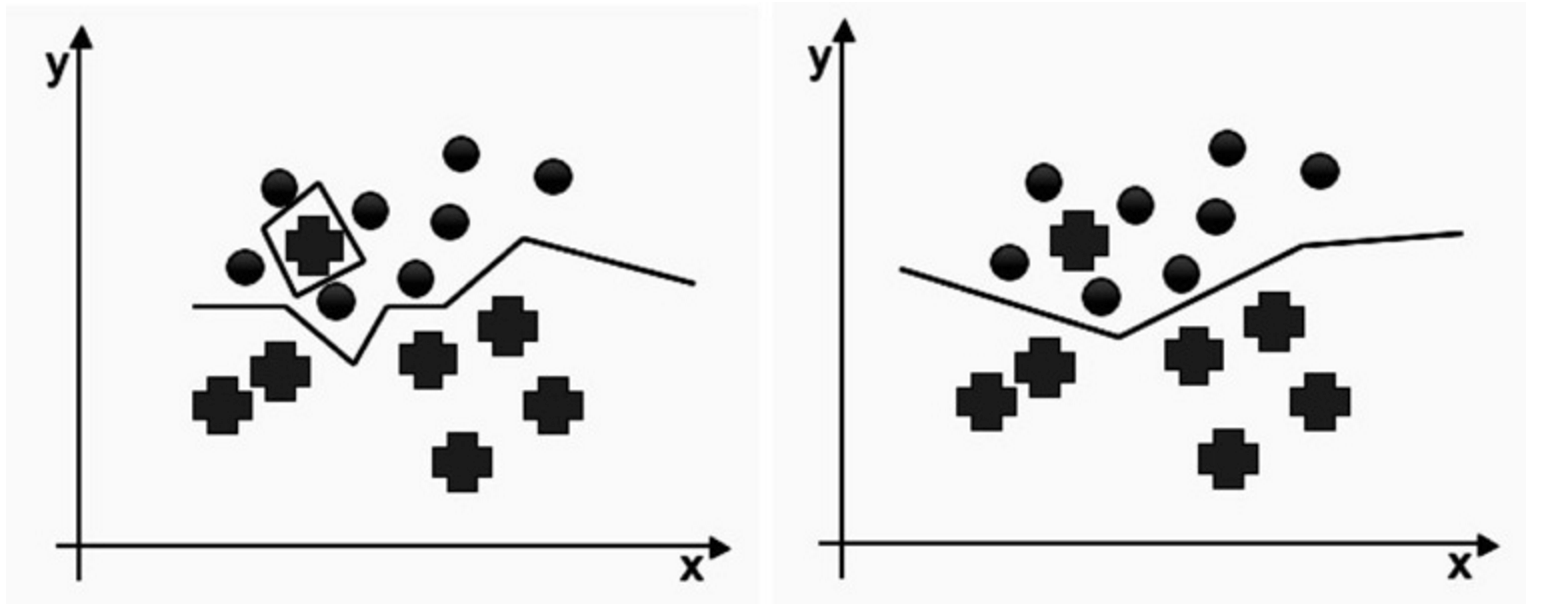
\includegraphics[width=0.9\linewidth]{knns-border}
    \end{center}

\end{frame}

\begin{frame}[fragile]{Python implementation of $k$-nearest neighbours}

\begin{onlyenv}<1>
\begin{pythoncode}
import numpy as np

def knn(k, data, categories, inputs):
  nb_inputs = np.shape(inputs)[0]
  closest = np.zeros(nb_inputs)

  for n in range(nb_inputs):
    # Compute distances
    distances = np.sum((data - inputs[n,:])\\2, axis=1)
    
    # Identify the nearest neighbours
    indices = np.argsort(distances, axis=0)

    classes = np.unique(categories[indices[:k]])
    
    if len(classes)==1:
        closest[n] = np.unique(classes)
    else:
        counts = np.zeros(max(classes) + 1)
        for i in range(k):
            counts[categories[indices[i]]] += 1
        closest[n] = np.argmax(counts, axis=0)
  return closest
\end{pythoncode}
\end{onlyenv}

\begin{onlyenv}<2>
    Alternatively, using \python{sklearn}:

\begin{pythoncode}
from sklearn import neighbors

knns = neighbors.KNeighborsClassifier(k)
knns.fit(data, categories)

predictions = knns.predict(inputs)
\end{pythoncode}

\end{onlyenv}

\begin{onlyenv}<3>
    Complete example, with the data above:

\begin{columns}
    \begin{column}{0.4\linewidth}
\begin{pythoncode}
""" data.csv:
2.2,1.3,0 -> circles
3.2,2.3,0
...

2.3,3.2,1 -> squares
0.3,0.6,1
...

2.8,3.5,2 -> stars
3.2,2.6,2
...
"""
\end{pythoncode}
        
    \end{column}
    \begin{column}{0.6\linewidth}
\begin{pythoncode}
from numpy import genfromtxt
from sklearn import neighbors

csv = genfromtxt('data.csv', delimiter=',')
data = csv[:,:2]
categories = csv[:,2]

inputs = [ [3.5,3], [1.5,3], [1.8,1.9] ]

k = 3
knns = neighbors.KNeighborsClassifier(k)
knns.fit(data, categories)

predictions = knns.predict(inputs)
print(predictions)

>>>  [2.  1.  1.]

\end{pythoncode}
    \end{column}
\end{columns}

\end{onlyenv}


\end{frame}

\begin{frame}{Choice of $k$ and weights}

\begin{center}
    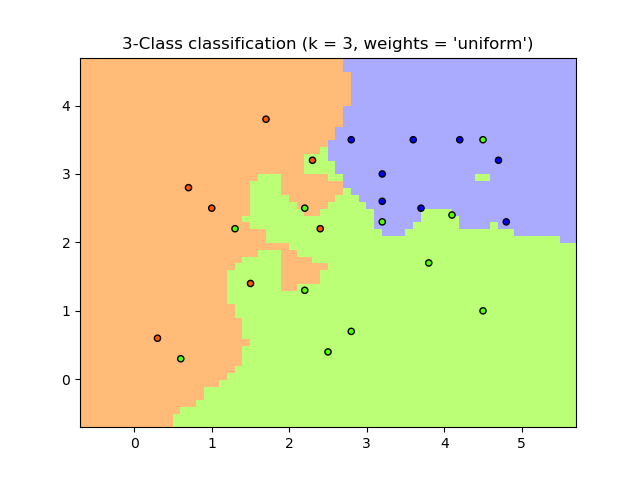
\includegraphics[width=0.45\linewidth]{knns_1}
    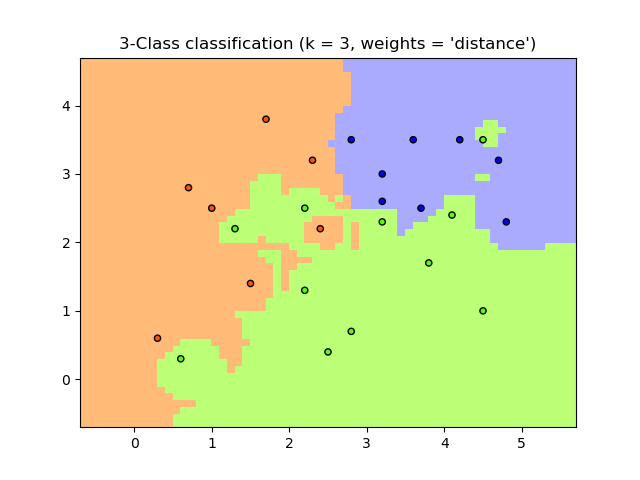
\includegraphics[width=0.45\linewidth]{knns_2}

    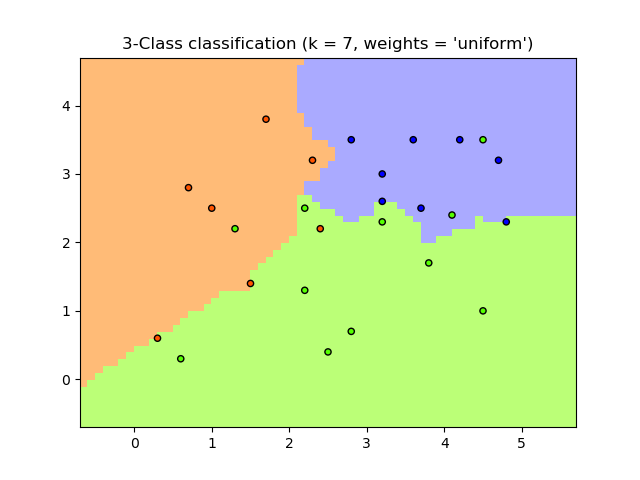
\includegraphics[width=0.45\linewidth]{knns_3}
    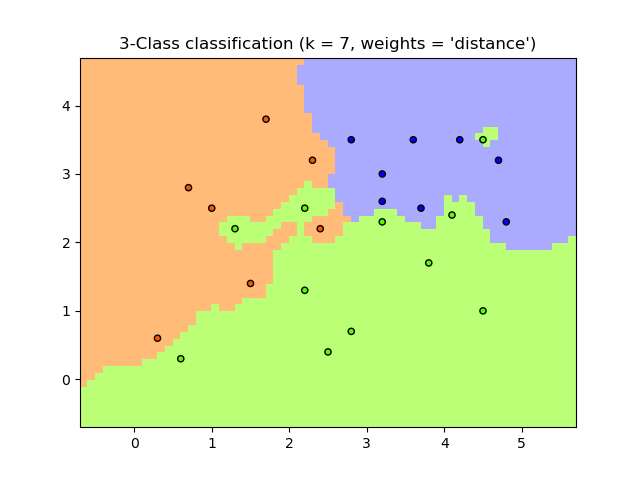
\includegraphics[width=0.45\linewidth]{knns_4}
\end{center}
\end{frame}


    \begin{frame}{$k$-nearest neighbours: summary}

\begin{itemize}
    \item<+-> $k$-nearest Neighbours usually does really well on a large number of
    classification problem, but can underperform near the classification
    boundary.

    \item<+-> might struggle with very large datasets, as it needs to calculate the
    distance to all training data every time you classify a new observation
    (some work around are available, relying on approximate distances and
    optimisation of the algorithmic code)

    \item<+-> commonly, the neighbours are weighted with the inverse of the
        distance $\frac{1}{d}$ to the observation (\ie closer neighbours have
        stronger influence). With \python{sklearn}:
        \python{neighbors.KNeighborsClassifier(k, weights='distance')}

\end{itemize}


\end{frame}

\begin{frame}{Support Vector Machines}

\only<1-3>{
A very popular classification algorithm introduced by Vapnik in 1992.

\pause

Often (but not always) provides very impressive classification
performance on reasonably sized datasets.

\pause
As opposed to $k$-nearest Neighbours, SVM are more difficult to understand
(although no knowledge of the algorithms internals is needed to use it).
}

 \only<4>{

SVMs do not work well on extremely large datasets, since (as we shall
see) the computations don't scale well with the number of training
examples, and so become computationally very expensive.

\begin{exampleblock}{Complexity}
Training a SVM requires $O(m^3)$\bubblemark{bigo} operations and $O(m^2)$
memory, with $m$ being the number of training samples. For example, if you
have 10,000 training samples, the training will take in the order of
$10^{12}$ operations (imagine you can do 100,000 operations/second, you
will need $10^8$ seconds $\equiv$ 3 years to train your SVM and $10^{12}$
memory units.
\end{exampleblock}

\bubble<1>[110][1.7][5cm]{bigo}{For more information on ``big-O notation'',
see \href{https://en.wikipedia.org/wiki/Time_complexity}{complexity of
algorithms}}

}
\end{frame}

\begin{frame}{SVM principle}

\only<1-2>{
Three different classification lines. All are correct, but is there any
reason why one is better than the others?
}

\only<3>{

The classifier in the middle is called the \textbf{maximum margin
classifier}.

The data points nearest the classifier are called \textbf{support
vectors}.

}


    \begin{center}
        \only<1>{
        \resizebox{0.3\linewidth}{!}{
            \begin{tikzpicture}[>=latex]

                \draw[thick, ->] (0,0) -> (5.2,0);
                \draw[thick, ->] (0,0) -> (0,4.2);

                \fill [hriSec2, opacity=0.5] (2.2,1.3) circle (2pt);
                \fill [hriSec2, opacity=0.5] (2.5,0.4) circle (2pt);
                \fill [hriSec2, opacity=0.5] (2.8,0.7) circle (2pt);
                \fill [hriSec2, opacity=0.5] (3.8,1.7) circle (2pt);
                \fill [hriSec2, opacity=0.5] (4.5,1.0) circle (2pt);
                \fill [hriSec2, opacity=0.5] (4.1,2.4) circle (2pt);

                \fill [hriSec3Comp, opacity=0.5] (2.3,3.2) rectangle +(3.5pt,3.5pt);
                \fill [hriSec3Comp, opacity=0.5] (0.7,2.8) rectangle +(3.5pt,3.5pt);
                \fill [hriSec3Comp, opacity=0.5] (1.7,3.8) rectangle +(3.5pt,3.5pt);
                \fill [hriSec3Comp, opacity=0.5] (1.0,2.5) rectangle +(3.5pt,3.5pt);
                \fill [hriSec3Comp, opacity=0.5] (2.2,2.5) rectangle +(3.5pt,3.5pt);
                \fill [hriSec3Comp, opacity=0.5] (1.3,2.2) rectangle +(3.5pt,3.5pt);

                \draw[dashed, ultra thick] (0,1.8) -- (4.9,2.8);

            \end{tikzpicture}
        }
        }
        \resizebox{0.3\linewidth}{!}{
            \begin{tikzpicture}[>=latex]

                \draw[thick, ->] (0,0) -> (5.2,0);
                \draw[thick, ->] (0,0) -> (0,4.2);

                \fill [hriSec2, opacity=0.5] (2.2,1.3) circle (2pt);
                \fill [hriSec2, opacity=0.5] (2.5,0.4) circle (2pt);
                \fill [hriSec2, opacity=0.5] (2.8,0.7) circle (2pt);
                \fill [hriSec2, opacity=0.5] (3.8,1.7) circle (2pt);
                \fill [hriSec2, opacity=0.5] (4.5,1.0) circle (2pt);
                \fill [hriSec2, opacity=0.5] (4.1,2.4) circle (2pt);

                \fill [hriSec3Comp, opacity=0.5] (2.3,3.2) rectangle +(3.5pt,3.5pt);
                \fill [hriSec3Comp, opacity=0.5] (0.7,2.8) rectangle +(3.5pt,3.5pt);
                \fill [hriSec3Comp, opacity=0.5] (1.7,3.8) rectangle +(3.5pt,3.5pt);
                \fill [hriSec3Comp, opacity=0.5] (1.0,2.5) rectangle +(3.5pt,3.5pt);
                \fill [hriSec3Comp, opacity=0.5] (2.2,2.5) rectangle +(3.5pt,3.5pt);
                \fill [hriSec3Comp, opacity=0.5] (1.3,2.2) rectangle +(3.5pt,3.5pt);

                \only<2->{
                \draw[red,opacity=0.5,line width=25pt] (0,0.65) -- (4.9,3.45);
                }
                \draw[dashed, ultra thick] (0,0.65) -- (4.9,3.45);

                \only<3>{
                    \draw [red, thick] (2.25,2.55) circle (5pt);
                    \draw [red, thick] (4.1,2.4) circle (5pt);
                    \draw [red, thick] (2.2,1.3) circle (5pt);

                }

            \end{tikzpicture}
        }
        \only<1>{
        \resizebox{0.3\linewidth}{!}{
            \begin{tikzpicture}[>=latex]

                \draw[thick, ->] (0,0) -> (5.2,0);
                \draw[thick, ->] (0,0) -> (0,4.2);

                \fill [hriSec2, opacity=0.5] (2.2,1.3) circle (2pt);
                \fill [hriSec2, opacity=0.5] (2.5,0.4) circle (2pt);
                \fill [hriSec2, opacity=0.5] (2.8,0.7) circle (2pt);
                \fill [hriSec2, opacity=0.5] (3.8,1.7) circle (2pt);
                \fill [hriSec2, opacity=0.5] (4.5,1.0) circle (2pt);
                \fill [hriSec2, opacity=0.5] (4.1,2.4) circle (2pt);

                \fill [hriSec3Comp, opacity=0.5] (2.3,3.2) rectangle +(3.5pt,3.5pt);
                \fill [hriSec3Comp, opacity=0.5] (0.7,2.8) rectangle +(3.5pt,3.5pt);
                \fill [hriSec3Comp, opacity=0.5] (1.7,3.8) rectangle +(3.5pt,3.5pt);
                \fill [hriSec3Comp, opacity=0.5] (1.0,2.5) rectangle +(3.5pt,3.5pt);
                \fill [hriSec3Comp, opacity=0.5] (2.2,2.5) rectangle +(3.5pt,3.5pt);
                \fill [hriSec3Comp, opacity=0.5] (1.3,2.2) rectangle +(3.5pt,3.5pt);

                \draw[dashed, ultra thick] (1.5,0) -- (3.2,4);

            \end{tikzpicture}
        }
        }
    \end{center}

\only<1-2> {

Intuitively, the line that is most distant to the training data is the
best division.

\onslide<2>{
The empty area near the division line is symmetric. It forms a bar in
2D space, a cylinder in 3D space, and a hyper-cylinder in n-D space.
}

}
\only<3> {
Two observations

\begin{itemize}

\item The margins should be as large as possible.
\item The support vectors are the most useful datapoints because they are
  the ones that we might get wrong.
\end{itemize}

}

\end{frame}

\begin{frame}{Linear classifier}

    \begin{center}
        \resizebox{0.3\linewidth}{!}{
            \begin{tikzpicture}[>=latex]

                \draw[thick, ->] (0,0) -> (5.2,0);
                \draw[thick, ->] (0,0) -> (0,4.2);

                \fill [hriSec2, opacity=0.5] (2.2,1.3) circle (2pt);
                \fill [hriSec2, opacity=0.5] (2.5,0.4) circle (2pt);
                \fill [hriSec2, opacity=0.5] (2.8,0.7) circle (2pt);
                \fill [hriSec2, opacity=0.5] (3.8,1.7) circle (2pt);
                \fill [hriSec2, opacity=0.5] (4.5,1.0) circle (2pt);
                \fill [hriSec2, opacity=0.5] (4.1,2.4) circle (2pt);

                \fill [hriSec3Comp, opacity=0.5] (2.3,3.2) rectangle +(3.5pt,3.5pt);
                \fill [hriSec3Comp, opacity=0.5] (0.7,2.8) rectangle +(3.5pt,3.5pt);
                \fill [hriSec3Comp, opacity=0.5] (1.7,3.8) rectangle +(3.5pt,3.5pt);
                \fill [hriSec3Comp, opacity=0.5] (1.0,2.5) rectangle +(3.5pt,3.5pt);
                \fill [hriSec3Comp, opacity=0.5] (2.2,2.5) rectangle +(3.5pt,3.5pt);
                \fill [hriSec3Comp, opacity=0.5] (1.3,2.2) rectangle +(3.5pt,3.5pt);

                \draw[dashed, ultra thick] (0,0.65) -- (4.9,3.45);

            \end{tikzpicture}
        }
        \hspace{2em}
        \only<4-5>{
        \resizebox{0.4\linewidth}{!}{
                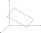
\includegraphics[width=\linewidth]{svm-hyperplane}
%            \begin{tikzpicture}[>=latex]
%
%                %\draw[help lines] (-1,-1) grid (5,4);
%                \draw[thick, ->] (0,0) -> (5.2,0);
%                \draw[thick, ->] (0,0) -> (0,4.2);
%                \draw[thick, ->] (0,0) -> (-1.5,-1.2);
%
%                \fill [hriSec2, opacity=0.5] (2.2,1.3) circle (2pt);
%                \fill [hriSec2, opacity=0.5] (2.5,0.4) circle (2pt);
%                \fill [hriSec2, opacity=0.5] (2.8,0.7) circle (2pt);
%                \fill [hriSec2, opacity=0.5] (3.8,1.7) circle (2pt);
%                \fill [hriSec2, opacity=0.5] (4.5,1.0) circle (2pt);
%                \fill [hriSec2, opacity=0.5] (4.1,2.4) circle (2pt);
%
%                \fill [hriSec3Comp, opacity=0.5] (2.3,3.2) rectangle +(3.5pt,3.5pt);
%                \fill [hriSec3Comp, opacity=0.5] (0.7,2.8) rectangle +(3.5pt,3.5pt);
%                \fill [hriSec3Comp, opacity=0.5] (1.7,3.8) rectangle +(3.5pt,3.5pt);
%                \fill [hriSec3Comp, opacity=0.5] (1.0,2.5) rectangle +(3.5pt,3.5pt);
%                \fill [hriSec3Comp, opacity=0.5] (2.2,2.5) rectangle +(3.5pt,3.5pt);
%                \fill [hriSec3Comp, opacity=0.5] (1.3,2.2) rectangle +(3.5pt,3.5pt);
%
%                \draw[dashed, ultra thick] (0,0.65) -- (4.9,3.45);
%                \draw[dashed, ultra thick] (0,0.65) -- (4.9,3.45);
%                \draw[dashed, ultra thick] (0,0.65) -- (4.9,3.45);
%                \draw[dashed, ultra thick] (0,0.65) -- (4.9,3.45);
%
%            \end{tikzpicture}
        }
        }
    \end{center}

\only<1>{

    A linear classifier for two categories (\textbf{binary classifier}) can be written as
    $f(\mathbf{x}) = \mathbf{w} \cdot \mathbf{x} + b$.

\begin{itemize}

    \item $\mathbf{w} \cdot \mathbf{x} = \sum_i w_i x_i$. This is called the
        scalar product or inner product. Can also be written as a matrix
        multiplication $\mathbf{w}^T\mathbf{x}$.
    \item $\mathbf{w}$ is a \textbf{weight vector}, tilting the line
    \item $\mathbf{x}$ is a data point (of dimension $n$)
    \item $b$ is a \textbf{bias}, lifting the line up along the $y$-axis
\end{itemize}

}
\only<2-3>{
    $\mathbf{w}$\bubblemark{weightvector} has to be calculated such that:
\[
f(\mathbf{x}) < 0 \Rightarrow \mathbf{x} \in \{\blacksquare\}
\]
\[
f(\mathbf{x}) > 0 \Rightarrow \mathbf{x} \in \{\circ\}
\]

\bubble<3>[115][0.8][4cm]{weightvector}{for kNNs, we have to carry along the training data; with a linear classifier, once $\mathbf{w}$ is found, we can discard the training data}
}



\only<4-5>{

    \begin{itemize}
        \item In 2D, the \textbf{discriminant} is a line
        \item In 3D, the discriminant is a plane
        \item In n-D\bubblemark{dimensions}, the discriminant is a hyperplane
    \end{itemize}

\bubble<5>[160][1][10cm]{dimensions}{the 'dimensions' are the \textbf{features} of our inputs, \eg for a human, the size, age, skin colour, gender...}
}

\end{frame}

\begin{frame}{Support vector classifier}

    \begin{center}
        \resizebox{0.3\linewidth}{!}{
            \begin{tikzpicture}[>=latex]

                \draw[thick, ->] (0,0) -> (5.2,0);
                \draw[thick, ->] (0,0) -> (0,4.2);

                \fill [hriSec2, opacity=0.5] (2.2,1.3) circle (2pt);
                \fill [hriSec2, opacity=0.5] (2.5,0.4) circle (2pt);
                \fill [hriSec2, opacity=0.5] (2.8,0.7) circle (2pt);
                \fill [hriSec2, opacity=0.5] (3.8,1.7) circle (2pt);
                \fill [hriSec2, opacity=0.5] (4.5,1.0) circle (2pt);
                \fill [hriSec2, opacity=0.5] (4.1,2.4) circle (2pt);

                \fill [hriSec3Comp, opacity=0.5] (2.3,3.2) rectangle +(3.5pt,3.5pt);
                \fill [hriSec3Comp, opacity=0.5] (0.7,2.8) rectangle +(3.5pt,3.5pt);
                \fill [hriSec3Comp, opacity=0.5] (1.7,3.8) rectangle +(3.5pt,3.5pt);
                \fill [hriSec3Comp, opacity=0.5] (1.0,2.5) rectangle +(3.5pt,3.5pt);
                \fill [hriSec3Comp, opacity=0.5] (2.2,2.5) rectangle +(3.5pt,3.5pt);
                \fill [hriSec3Comp, opacity=0.5] (1.3,2.2) rectangle +(3.5pt,3.5pt);


                \draw[red,opacity=0.5,line width=25pt] (0,0.65) -- (4.9,3.45);
                \draw[dashed, ultra thick] (0,0.65) -- (4.9,3.45);

                    \draw [red, thick] (2.25,2.55) circle (5pt);
                    \draw [red, thick] (4.1,2.4) circle (5pt);
                    \draw [red, thick] (2.2,1.3) circle (5pt);




            \end{tikzpicture}
        }
    \end{center}


In a SVM, we want to \textbf{maximise the margin} $M$. We can rewrite the linear
classifier.
    
If $\mathbf{w}^T\mathbf{x} + b \geq M$, then an observation belongs to
$\blacksquare$, for $\mathbf{w}^T\mathbf{x} + b \leq −M$, it belongs to
$\circ$.

\pause
A point $\mathbf{x}^\blacksquare$ that lies on the $\blacksquare$ class
boundary line, \ie $\mathbf{w}^T\mathbf{x}^\blacksquare + b = M$, is
a \textbf{support vector}.


\end{frame}

\begin{frame}{Finding the optimal classifier}

The problem is to find the \textbf{optimal} values for $\mathbf{w}$ and
$b$.

The classifier needs to satisfy two conditions

\begin{itemize}

\item It needs to correctly classify the training data,
\item and needs the margin from the classifier to be as large as possible.
\end{itemize}

\pause

A \textbf{quadratic programming solver} is used to find the optimal
values for $\mathbf{w}$ and $b$.

{\footnotesize \href{http://www.robots.ox.ac.uk/~az/lectures/ml/lect2.pdf}{Oxford lecture on SVM} to learn more about the mathematical
    formulation and the \emph{perceptron algorithm}.}

\end{frame}

\begin{frame}{Transformation of data}

\begin{itemize}

    \item Unfortunately, \emph{all this still assumes that the data is linearly
        separable}. But what if it is not, and we are not prepared for a few
  misclassifications?
\item The solution is to \textbf{transform} the data: move data points in
  the n-D space until the training data is linearly separable again
\end{itemize}

    \begin{center}
        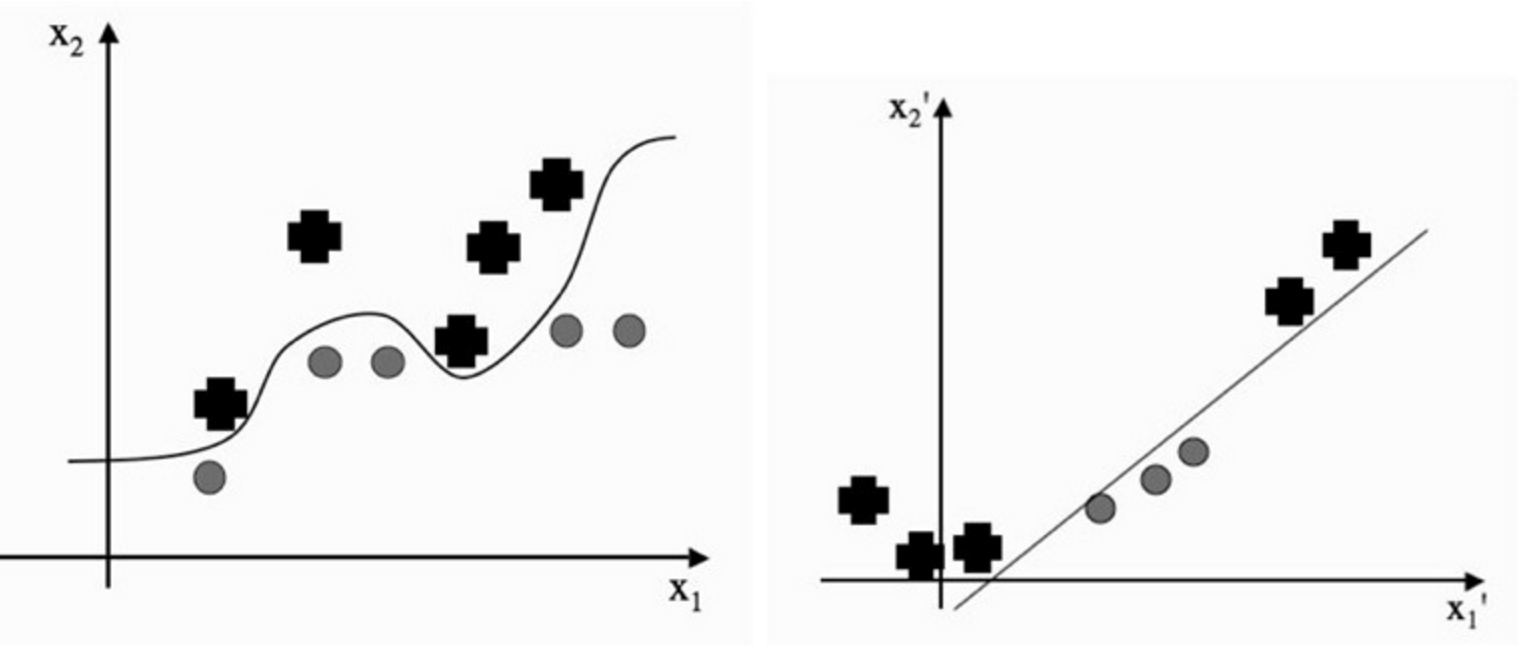
\includegraphics[width=0.8\linewidth]{svm-kernels}
    \end{center}
\end{frame}

\begin{frame}{Feature maps}

We can transform data points (= move them) or even add more dimensions.  using
some function $\theta(\mathbf{x}_i)$ from input $\mathbf{x}_i$. $\theta$ is a \textbf{feature
map}.

\only<1>{
Example:
    \[
        \theta(\mathbf{x}_i) = [\mathbf{x}_i, \mathbf{x}^2_i]
    \]

\begin{center}
    
\includegraphics[width=0.8\linewidth]{svm-kernels-separation}
\end{center}

$\rightarrow$ now, linearly separable
}

\only<2>{
Example:
    \[
        \theta(<x_i, y_i>) = [x_i, y_i, x^2_i + y^2_i]
    \]

\begin{center}
    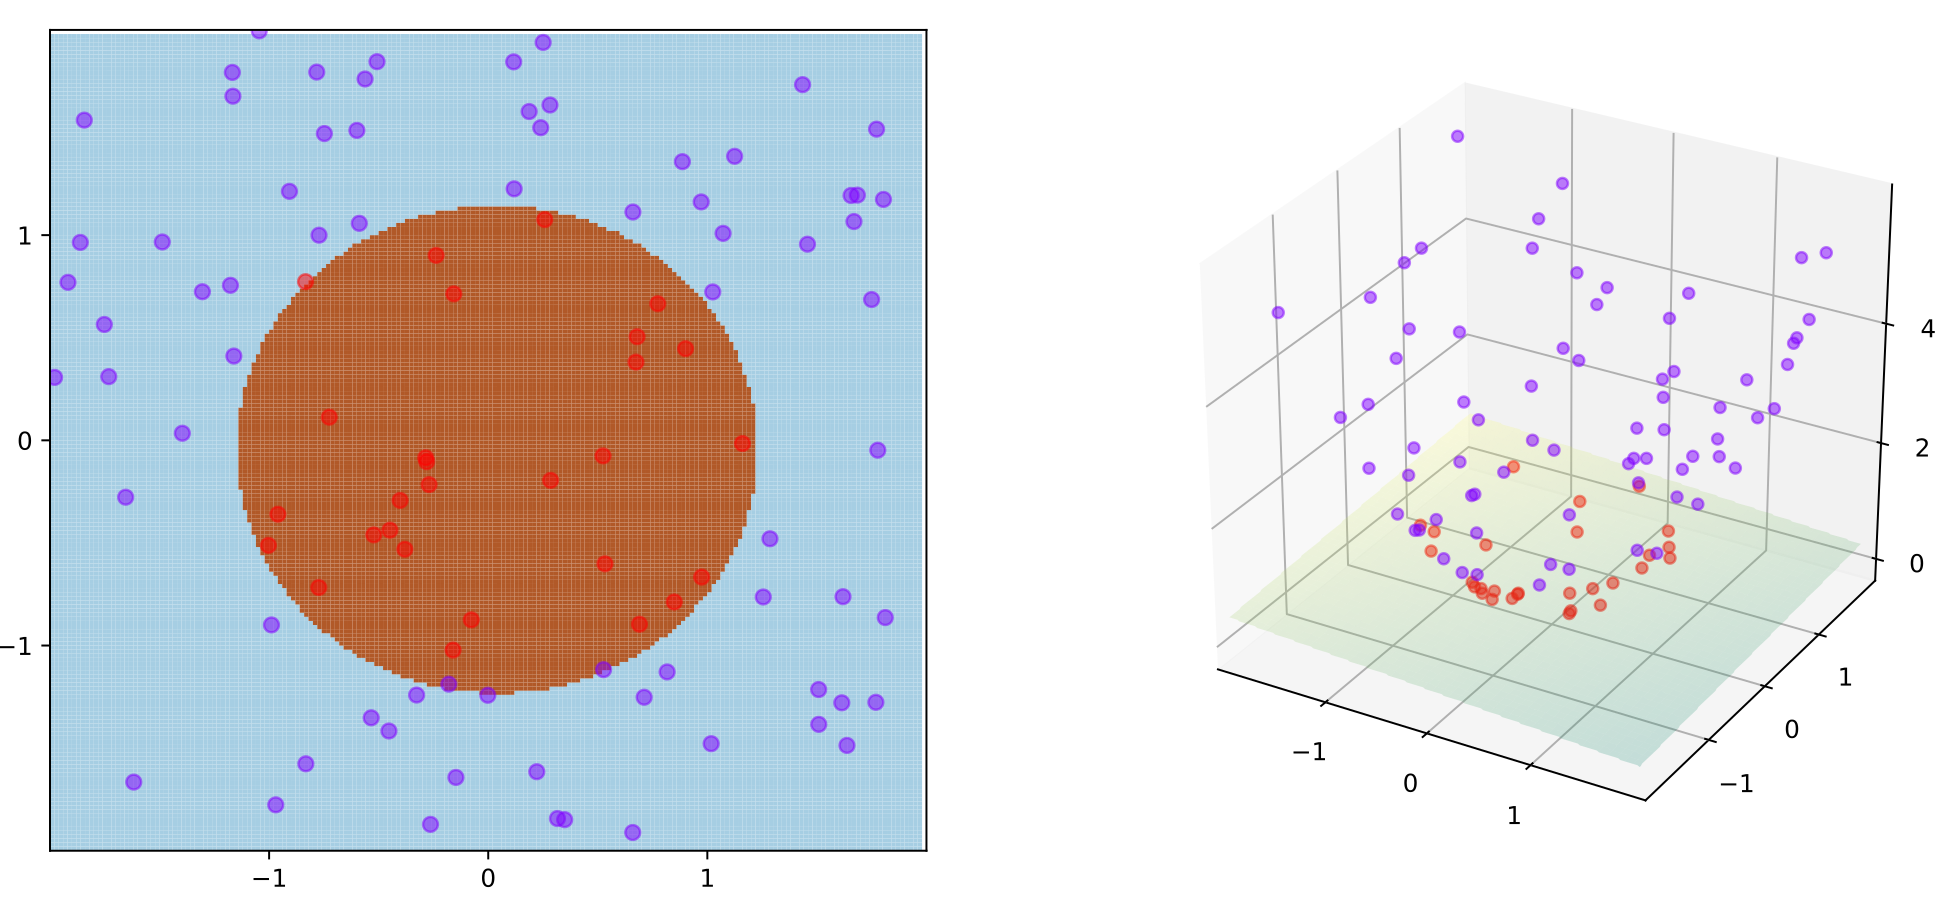
\includegraphics[width=0.7\linewidth]{svm-kernel-3d}
\end{center}

$\rightarrow$ now, linearly separable
}
\only<3>{


If we know something about the structure of the data, then we might be able to identify
feature maps that would be effective.

Often however we do not have such domain knowledge.
}

\end{frame}

\begin{frame}{The kernel trick}

\[
        \theta: \mathbf{x} \rightarrow  \theta(\mathbf{x}), \mathbb{R}^d \rightarrow \mathbb{R}^D
\]

\begin{itemize}
    \item Simply map $\mathbf{x}$ to $\theta(\mathbf{x})$ where data is separable
    \item Solve for $\mathbf{w}$ in high dimensional space $\mathbb{R}^D$
    \item If $D >> d$ then there are many more parameters to learn for $\mathbf{w}$. Can this be avoided?
\end{itemize}

    \href{http://www.robots.ox.ac.uk/~az/lectures/ml/lect3.pdf}{It can be shown that} you actually do not need to calculate explicitely $\theta(\mathbf{x})$. Instead, you only need $\theta(\mathbf{x}_i)^T \theta(\mathbf{x}_j)$ (with $\mathbf{x}_i$ the training data) to compute $\mathbf{w}$.

    \pause

    We call the \textbf{kernel function} $K(\mathbf{x}_i,\mathbf{x}_j) = \theta(\mathbf{x}_i)^T \theta(\mathbf{x}_j)$.
    The SVM classifier can be learnt and applied with only $K$, and the complexity depends only on $N$ (size of training data), not on $D$.


\end{frame}

\begin{frame}{Standard kernels}

\begin{itemize}

    \item \textbf{Polynomials} up to some degree $s$ in the
  elements $x_k$ of the input vector (\eg $x^3_3$ or $x_1 x_4$). This can be written as:

    \[
        K(x, y) = (1 + x^Ty)^s
    \]

\item \textbf{Sigmoid functions} of the $x_k$ with parameters $\kappa$ and $\delta$, and
  kernel:
    \[
        K(x, y) = tanh(\kappa x^T y - \delta)
    \]
\item \textbf{Radial basis function} expansions of the $x_k$ with parameter $\sigma$
  and kernel:
    \[
        K(x, y) = exp(- \frac{(x-y)^2}{2\sigma^2})
    \]

(a Gaussian kernel)

\end{itemize}

\end{frame}

\begin{frame}{Comparison of kernel functions}
    \begin{center}
        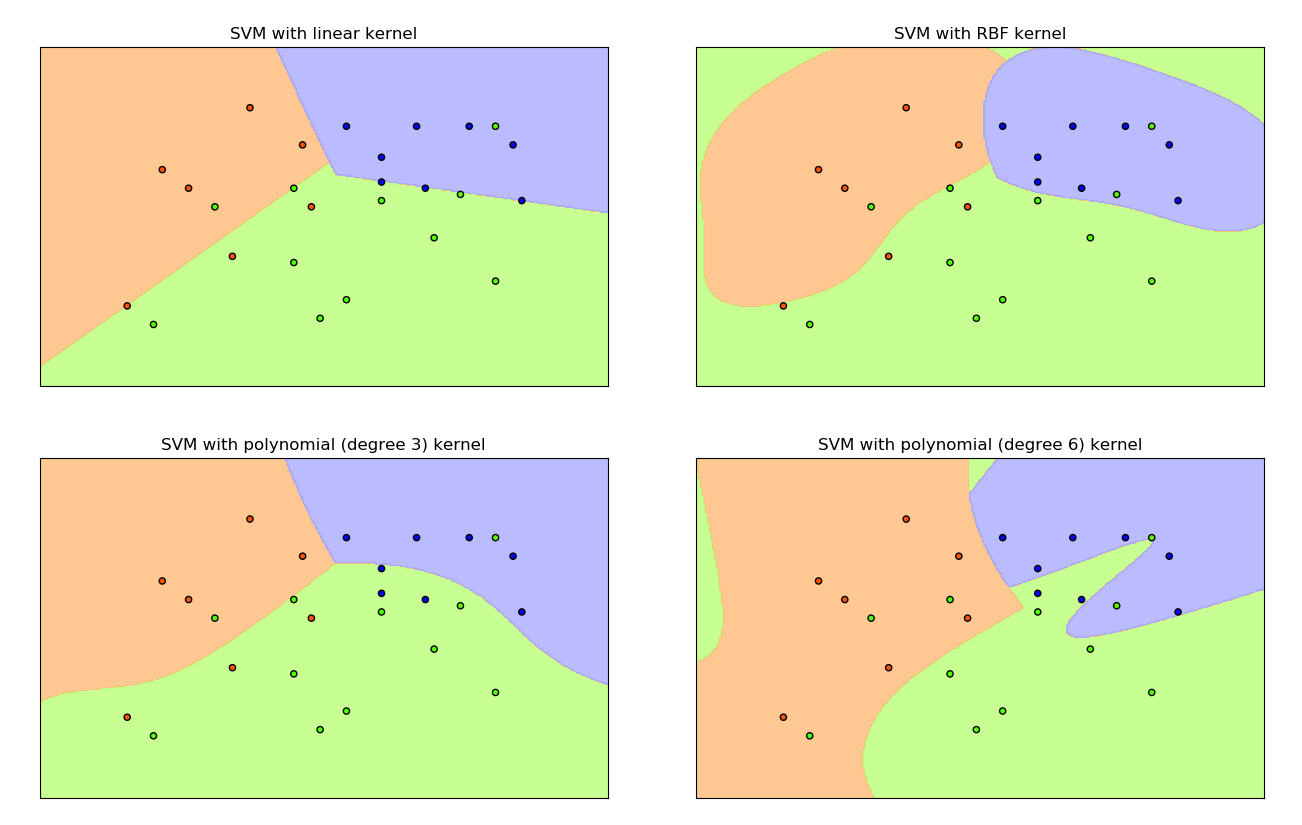
\includegraphics[width=\linewidth]{svm_comparison}
    \end{center}
\end{frame}

\begin{frame}[fragile]{Python implementation of Support Vector Machine}

\begin{onlyenv}<1>

\begin{pythoncode}
from sklearn import svm

C = 1.0  # SVM regularization parameter ~~ 'how acceptable are misclassification'
clf = svm.SVC(kernel='linear', C=C) # kernel='poly', 'rbf', 'sigmoid'...

clf.fit(data, categories)

predictions = clf.predict(inputs)
\end{pythoncode}

\end{onlyenv}

\begin{onlyenv}<2>
    Complete example, with our data:

\begin{columns}
    \begin{column}{0.4\linewidth}
\begin{pythoncode}
""" data.csv:
2.2,1.3,0 -> circles
3.2,2.3,0
...

2.3,3.2,1 -> squares
0.3,0.6,1
...

2.8,3.5,2 -> stars
3.2,2.6,2
...
"""
\end{pythoncode}
        
    \end{column}
    \begin{column}{0.6\linewidth}
\begin{pythoncode}
from numpy import genfromtxt
from sklearn import svm

csv = genfromtxt('data.csv', delimiter=',')
data = csv[:,:2]
categories = csv[:,2]


inputs = [ [3.5,3], [1.5,3], [1.8,1.9] ]

clf = svm.SVC(kernel='rbf',
              gamma = 0.7,
              C=1.0)
clf.fit(data, categories)

predictions = clf.predict(inputs)
print(predictions)

>>>  [2.  1.  0.]

\end{pythoncode}
    \end{column}
\end{columns}

\end{onlyenv}


\end{frame}

\begin{frame}{Choosing the kernel}


Choosing which kernel to use and the parameters in these kernels is a
tricky problem. While there is some theory based on something known as
the Vapnik--Chernik dimension that can be applied, most people just
experiment with different values and find one that works.

\end{frame}



\begin{frame}{The iris data set}

Classifies three species of irises (flowers) on the bases of four
properties

\begin{itemize}

\item Sepal length, sepal width, petal length, petal width
\end{itemize}


    \begin{center}
        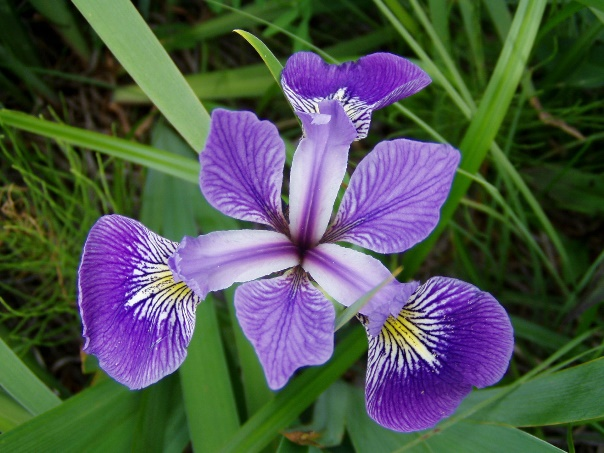
\includegraphics[width=0.35\linewidth]{iris}
        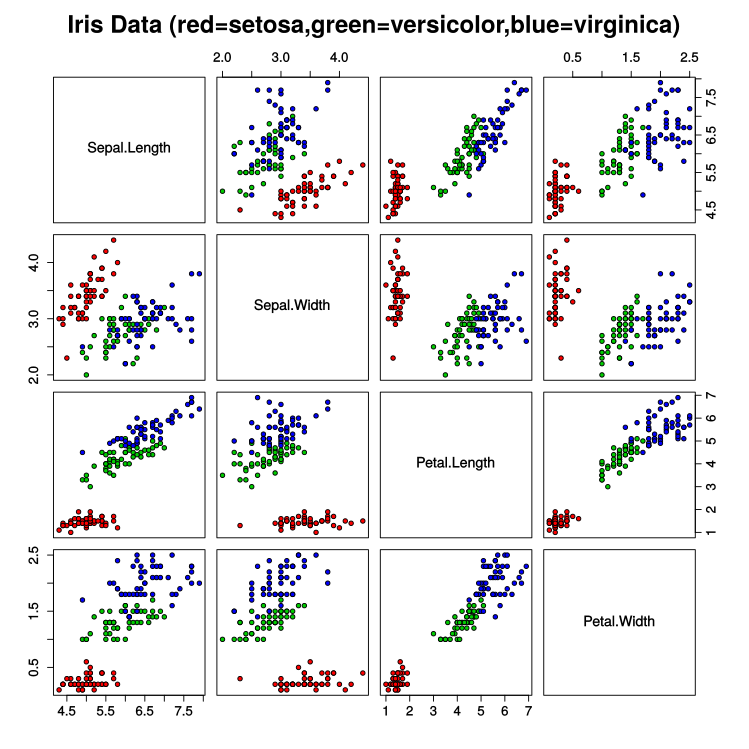
\includegraphics[width=0.5\linewidth]{iris-classification}
    \end{center}

\end{frame}

\begin{frame}{Clustering vs classification}

\textbf{Clustering} is sometimes confused with \textbf{classification}.  (often
    because some algorithms have similar names,e.g. \emph{k-means clustering}
    and \emph{k-nearest neighbours}).

\textbf{Clustering} starts from unlabelled data points and tries to find
    $k$ clusters in the data $\rightarrow$ \textbf{unsupervised learning}.


$\rightarrow$ Used to find patterns in the data.

    \begin{center}
        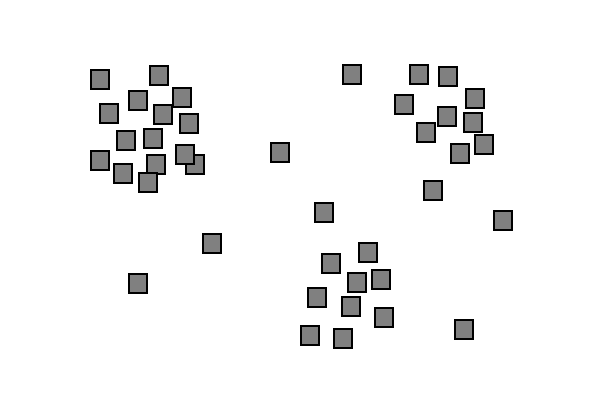
\includegraphics[width=0.3\linewidth]{clustering-0}
        $\rightarrow$
        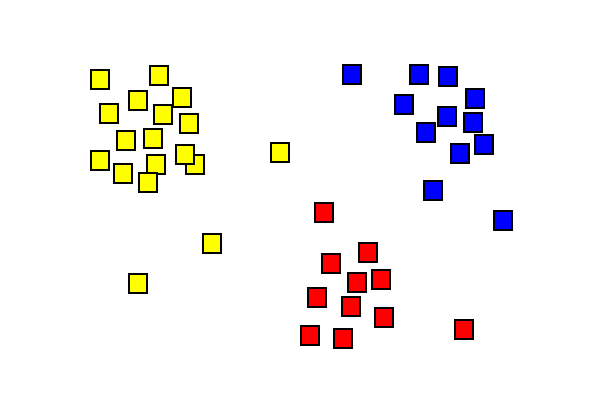
\includegraphics[width=0.3\linewidth]{clustering-1}
    \end{center}


    \textbf{Classification} starts from training data ($\rightarrow$
    \textbf{supervised learning}), and attempts to correctly classify an
    unknown observation.

\end{frame}

%%%%%%%%%%%%%%%%%%%%%%%%%%%%%%%%%%%%%%%%%%%%%%%%%%%%%%%%%%%%%%%%%%%%%%%
%%%%%%%%%%%%%%%%%%%%%%%%%%%%%%%%%%%%%%%%%%%%%%%%%%%%%%%%%%%%%%%%%%%%%%%
%%%%%%%%%%%%%%%%%%%%%%%%%%%%%%%%%%%%%%%%%%%%%%%%%%%%%%%%%%%%%%%%%%%%%%%

\section[Classifying social signal]{How to classify social signal?}

\begin{frame}{How to classify social signals?}

    Raw signals will in most cases require pre-processing to extract
features.

The raw social signal (audio or video) requires pre-processing\bubblemark{preprocessing} to
extract between 10 and over a 1000 \textbf{features}.

\begin{itemize}

    \item A raw signals contains too much data, and cannot be fed to the
      classifier immediately.

        \begin{center}
            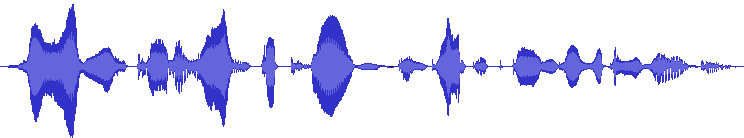
\includegraphics[width=0.5\linewidth]{rawaudio}
        \end{center}

    \item Pre-processing extracts feature data which is relevant for the
  information which we are after (pitch, volume/energy, duration,
  formant frequencies, \ldots{})
    \item These features then form the input for the classifier.
\end{itemize}

    {\footnotesize
For more information see, for example, Liang et al. (2005)
\href{http://ieeexplore.ieee.org/xpls/icp.jsp?arnumber=1571239}{Feature
analysis and extraction for audio automatic classification}, Systems,
Man and Cybernetics, 2005 IEEE International Conference on.
    }

\bubble<2>[50][0.7][5cm]{preprocessing}{An exception to this are Convolutional Neural
    Networks, which can deal with unprocessed data}

\end{frame}

\begin{frame}{Example: recognising gender from speech}

Can we automatically recognise someone's gender from speech?

3,168 recorded voice samples, collected from male and female speakers.

\begin{itemize}

\item Examples from the database: male (US), female (US), male (Scotish)
\end{itemize}

    \begin{center}
    \video[1]{1cm}{figs/male-us.mp4}\hspace{0.3em}
    \video[1]{1cm}{figs/male-scottish.mp4}\hspace{0.3em}
    \video[1]{1cm}{figs/female-us.mp4}
    \end{center}


The voice samples are pre-processed by acoustic analysis in R using the
{\tt seewave}, {\tt warbleR} and {\tt tuneR} packages, with an analysed frequency range of
0hz-280Hz (fundamental frequency of human speech).

\begin{itemize}

\item Extracted 20 features.
\end{itemize}

    \source{https://www.kaggle.com/primaryobjects/voicegender}{data and more information}


\end{frame}

\begin{frame}{The 20 features used for gender classification}

    \only<1>{
\begin{itemize}

\item \textbf{meanfreq}: mean frequency (in kHz)
\item \textbf{sd}: standard deviation of frequency
\item \textbf{median}: median frequency (in kHz)
\item \textbf{Q25}: first quantile (in kHz)
\item \textbf{Q75}: third quantile (in kHz)
\item \textbf{IQR}: interquantile range (in kHz)
\item \textbf{skew}: skewness (see note in specprop description)
\item \textbf{kurt}: kurtosis (see note in specprop description)
\item \textbf{sp.ent}: spectral entropy
\item \textbf{sfm}: spectral flatness
\item \textbf{mode}: mode frequency
\item \textbf{centroid}: frequency centroid (see specprop)
\item \textbf{peakf}: peak frequency (frequency with highest energy)
\end{itemize}
}
    \only<2>{
\begin{itemize}

\item \textbf{meanfun}: average of fundamental frequency measured across
  acoustic signal
\item \textbf{minfun}: minimum fundamental frequency measured across
  acoustic signal
\item \textbf{maxfun}: maximum fundamental frequency measured across
  acoustic signal
\item \textbf{meandom}: average of dominant frequency measured across
  acoustic signal
\item \textbf{mindom}: minimum of dominant frequency measured across
  acoustic signal
\item \textbf{maxdom}: maximum of dominant frequency measured across
  acoustic signal
\item \textbf{dfrange}: range of dominant frequency measured across acoustic
  signal
\item \textbf{modindx}: modulation index. Calculated as the accumulated
  absolute difference between adjacent measurements of fundamental
  frequencies divided by the frequency range
\end{itemize}
}

\end{frame}

\begin{frame}{Example: recognising gender from speech}

    \begin{center}
        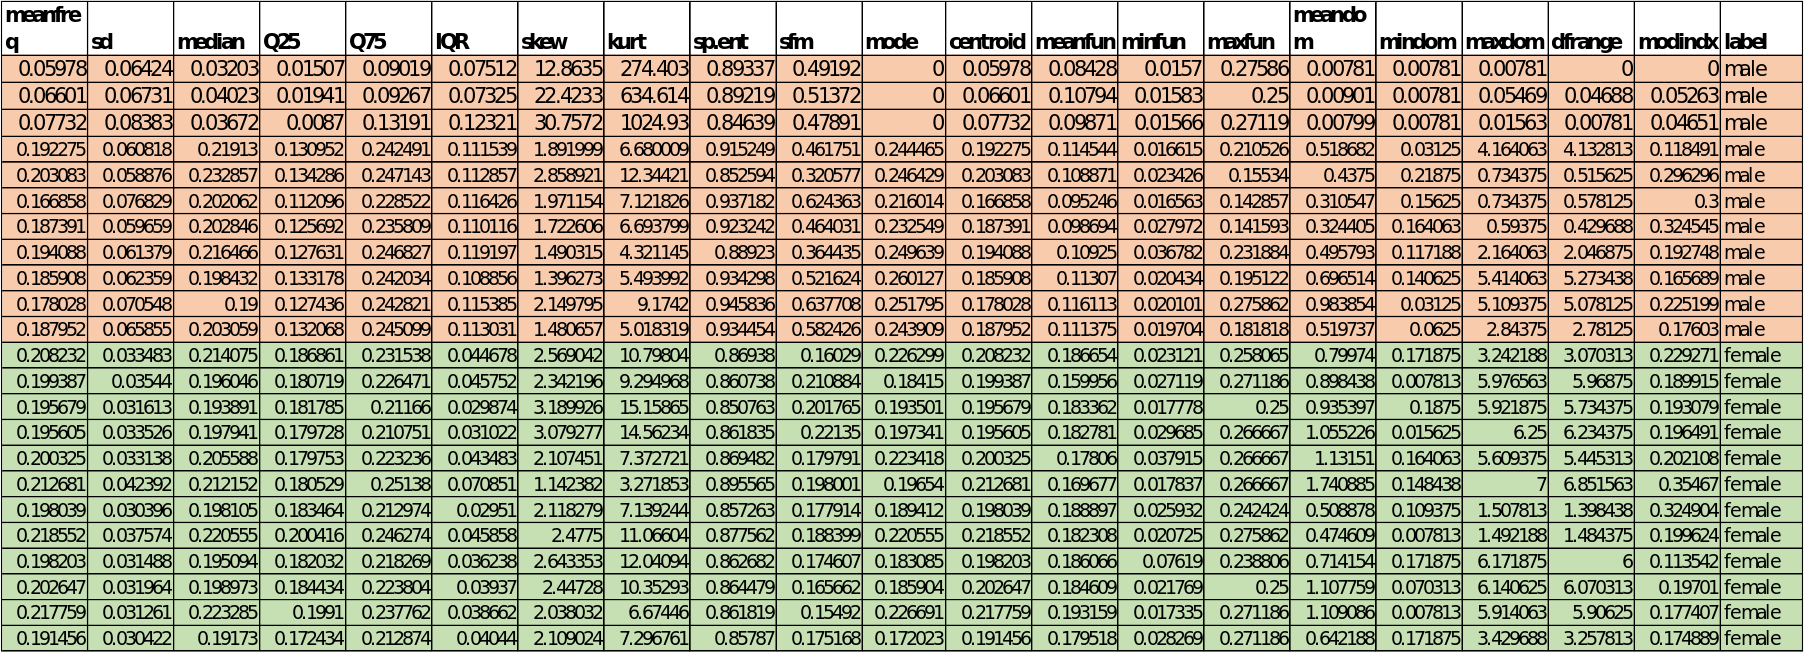
\includegraphics[width=\linewidth]{vector-gender-voice}
    \end{center}
\end{frame}

\begin{frame}{Example: recognising gender from speech}

Performance

\begin{itemize}

\item kNN (k = 7): 97.8\% classified correctly.
\item SVM: 97.5\% classified correctly.
\end{itemize}

Recognising gender from speech is easy and robust.

\begin{itemize}

\item All classification algorithms can deal with this problem (at least all
  the ones I tried).
\end{itemize}

\end{frame}

\begin{frame}{Conclusion}

Social signal processing is extracting relevant information from the
social environment.

Some work relatively well

\begin{itemize}

\item Face \textbf{detection}, voice activity detection, gender
  classification, \ldots{}
\end{itemize}

Some work, but need improvement

\begin{itemize}

\item Gaze detection, basic emotion recognition, face \textbf{recognition},
  speech recognition, \ldots{}
\end{itemize}

But still many open problems remaining

\begin{itemize}

\item Complex real-word affect and emotion recognition (e.g.~embarrassment,
  pride).
\item Speech recognition for atypical speakers (children, elderly),
  multi-party interaction, \ldots{}
\end{itemize}

\end{frame}


\begin{frame}{}
    \begin{center}
        \Large
        That's all, folks!\\[2em]
        \normalsize
        Questions:\\
        Portland Square A216 or \url{severin.lemaignan@plymouth.ac.uk} \\[1em]

        Slides:\\ \href{https://github.com/severin-lemaignan/module-mobile-and-humanoid-robots}{\small github.com/severin-lemaignan/module-mobile-and-humanoid-robots}

    \end{center}
\end{frame}



\end{document}
